% ----------------------------------------------------------------------
%                   Original Latex File from Joseph Roche's PhD (2012)
% ----------------------------------------------------------------------

%Latext thesis template from Harish Bhanderi's PhD/MPhil template, then Uni Cambridge
% http://www-h.eng.cam.ac.uk/help/tpl/textprocessing/ThesisStyle/

%: Style file for Latex
% Most style definitions are in the external file PhDthesisPSnPDF.
% In this template package, it can be found in ./Latex/Classes/
\documentclass[a4paper,oneside,12pt]{Latex/Classes/PhDthesisPSnPDF}
\setcitestyle{numbers}
%Change "oneside" to "twoside" for final submission-grade thesis after viva/corrections

\usepackage[subpreambles=true]{standalone} %For using chapter files properly
\usepackage{amsbsy}
\usepackage{amsmath}
\usepackage{booktabs}
\usepackage{caption}
\usepackage{comment}
\usepackage{epstopdf}
\usepackage{fancyhdr}
\usepackage{gensymb}
\usepackage{hyperref}
\usepackage[utf8]{inputenc}
\usepackage{lineno}
\usepackage{lscape}
\usepackage{multirow}
%\usepackage[round]{natbib}
\usepackage{notoccite}
\usepackage{paralist}
\usepackage{quotchap}
\usepackage{rotating}
\usepackage{setspace}
\usepackage{sidecap}
\usepackage{siunitx}
\usepackage{subcaption}
\usepackage{textcomp}
%\usepackage{titlesec}
\usepackage{url}
\usepackage{wrapfig}
\usepackage{wtmmPkg}
\usepackage{xspace}

\usepackage[font={footnotesize}]{caption}
\usepackage[capitalise]{cleveref}
%\usepackage[inner=3.5cm, outer=2cm,top=3.3cm, bottom=2.0cm, footskip=1cm, twoside, includeall]{geometry}
\usepackage[bindingoffset=1.5cm, right=2cm, left=2cm, top=3.3cm, bottom=2.0cm, footskip=1.0cm]{geometry}

%\usepackage[twoside, bindingoffset=3.5cm, margin=2cm,includeall]{geometry}
\usepackage[font={footnotesize}]{subcaption}

\Crefname{figure}{Fig.}{Figs.}% {<type>}{<singular>}{<plural>}

%\renewcommand{\bibpreamble}{\begin{multicols}{2}}
%\renewcommand{\bibpostamble}{\end{multicols}}

% David McKenna: Macro to make the Specs Tables align better
\usepackage{array}
\usepackage{ragged2e}
\newcolumntype{L}[1]{>{\raggedright\let\newline\\\arraybackslash\hspace{0pt}}m{#1}}

%\usepackage{geometry}

%%% Added by DOF Jan 2018
% This gets rid of ugly hyperlink boxes for pdf versions
% Replaces boxes with changed text colour.
% Looks way better
\usepackage{xcolor}
%% for pdf use this:
  \hypersetup{
      colorlinks,
      linkcolor={red},
      citecolor={blue!80!black},
      urlcolor={blue!80!black}
  }
%% for printing use this:
%\hypersetup{
%    colorlinks,
%    linkcolor=.,
%    citecolor=.,
%    urlcolor=.
%      }

\creflabelformat{equation}{#2\textup{#1}#3}

%\usepackage{showframe}

%%%
% Added by DOF Jan 2018 to make nicer chapter numbers
% comment out next lines to revert to default
% (Don't forget to uncomment titlesec package above!!!!)
%%%
\usepackage{color}
\definecolor{RoyalRed}{RGB}{157,16, 45}
%\renewcommand{\sfdefault}{mdugm} %Garamond
\usepackage[ ]{titlesec}  %
\titleformat{\chapter}[display]
  { \normalsize \huge  \color{RoyalRed}}
  {\flushright \normalsize \color{RoyalRed} \MakeUppercase {} \vspace{-45mm} \hspace{1 ex} { \fontsize{55}{55}\selectfont \color{RoyalRed} \sffamily  \thechapter }} {10 pt}{\raggedleft \Huge}
\titlespacing{\chapter}{0pt}{50pt}{5mm}%


%Added by SM 13 Sep 2011 to get backref to read ''Cited on page''
   \usepackage{Latex/StyleFiles/backrefx}
       \renewcommand{\backrefpagesname}{Cited on page~}
       \renewcommand{\backrefpagesnames}{Cited on pages~}

\newcommand{\BibTeX}{\textsc{Bib}\TeX}
\newcommand{\etal}{{\it et al.}}

% Definitions for equations
\newcommand{\arcsec}{^{\prime\prime}}
\newcommand{\arcmin}{^{\prime}}
%\def\ion#1#2{#1$\;${\small\rm\@Roman{#2}}\relax}
\DeclareRobustCommand{\ion}[2]{%
\relax\ifmmode
\ifx\testbx\f@series
{\mathbf{#1\,\mathsc{#2}}}\else
{\mathrm{#1\,\mathsc{#2}}}\fi
\else\textup{#1\,{\mdseries\textsc{#2}}}%
\fi}

\newcommand{\subion}{ {_{ion}} }
\newcommand{\sube}{ {_{e}} }
\newcommand{\subj}{ {_{j}} }
\newcommand{\subi}{ {_{i}} }
\newcommand{\ji}{ {_{j,i}} }
\newcommand{\rt}{ {$R(T)$} }
\newcommand{\rlam}{ {$R(\lambda)$} }
\newcommand{\rsun}{R$_{\odot}$}
\newcommand{\rmd}{ {\ \mathrm d} }
\renewcommand{\vec}[1]{ {\mathbf #1} }
\newcommand{\uvec}[1]{ \hat{\mathbf #1} }
\newcommand{\pder}[2]{ \f{\partial #1}{\partial #2} }
\newcommand{\grad}{ {\bf \nabla } }
\newcommand{\curl}{ {\bf \nabla} \times}
\newcommand{\vol}{ {\mathcal V} }
\newcommand{\bndry}{ {\mathcal S} }
\newcommand{\dv}{~{\mathrm d}^3 x}
\newcommand{\da}{~{\mathrm d}^2 x}
\newcommand{\dl}{~{\mathrm d} l}
\newcommand{\dt}{~{\mathrm d}t}
\newcommand{\intv}{\int_{\vol}^{}}
\newcommand{\inta}{\int_{\bndry}^{}}
\newcommand{\avec}{ \vec A}
\newcommand{\ap}{ \vec A_p}
\newcommand{\bb}{ \vec B}
\newcommand{\jj}{ \vec j}
\newcommand{\rr}{ \vec r}
\newcommand{\xx}{ \vec x}

% Definitions for the journal names
\newcommand{\adv}{    {\it Advances in Space Research}}
\newcommand{\annG}{   {\it Annales Geophysicae}}
\newcommand{\aap}{    {\it Astronomy \& Astrophysics}}
\newcommand{\aaps}{   {\it Astronomy \& Astrophysics Supplemental}}
\newcommand{\aapr}{   {\it Astronomy \& Astrophysics Review}}
\newcommand{\ag}{     {\it Ann. Geophys.}}
\newcommand{\aj}{     {\it Astronomical Journal}}
\newcommand{\apj}{    {\it Astrophysical Journal}}
\newcommand{\apjs}{    {\it Astrophysical Journal Supplemental Series}}
\newcommand{\apjl}{   {\it Astrophysical Journal Letters}}
\newcommand{\apss}{   {\it Astrophysics \& Space Science}}
\newcommand{\cjaa}{   {\it Chinese Journal Astronomy \& Astrophysics}}
\newcommand{\gafd}{   {\it Geophysical and Astrophysical Fluid Dynamics}}
\newcommand{\grl}{    {\it Geophysical Research Letters}}
\newcommand{\ijga}{   {\it International Journal of Geomagnetism and Aeronomy}}
\newcommand{\jastp}{  {\it Journal of Atmospheric and Solar-Terrestrial Physics}}
\newcommand{\jgr}{    {\it Journal of Geophysical Research}}
\newcommand{\mnras}{  {\it Monthly Notices of the Royal Astronomical Society}}
\newcommand{\nat}{    {\it Nature}}
\newcommand{\pasp}{   {\it Publications of the Astronomical Society of the Pacific}}
\newcommand{\pasj}{   {\it Publications of the Astronomical Society of Japan}}
\newcommand{\pra}{    {\it Physical Review A}}
\newcommand{\pre}{    {\it Physical Review E}}
\newcommand{\solphys}{{\it Solar Physics}}
\newcommand{\sovast}{ {\it Soviet Astronomy}}
\newcommand{\ssr}{    {\it Space Science Reviews}}
\newcommand{\araa}{  {\it Annual Review of Astronomy \& Astrophysics}}
\newcommand{\memsai}{ {\it Memorie della Societa Astronomia Italiana}}
\newcommand{\planss}{ {\it Planetary and Space Science} }
\newcommand{\actaa}{ {\it Acta Astronomica} }
\newcommand{\zap}{ {\it Zeitschrift für Astrophysik} }

%Definitions JHT
\newcommand{\ztfg}{$g$}
\newcommand{\ztfr}{$r$}
\newcommand{\ztfi}{$i$}

%: Macro file for Latex
% Macros help you summarise frequently repeated Latex commands.
% Here, they are placed in an external file /Latex/Macros/MacroFile1.tex
% An macro that you may use frequently is the figuremacro (see introduction.tex)

%\DeclareUnicodeCharacter{2010}{-}
% This file contains macros that can be called up from connected TeX files
% It helps to summarise repeated code, e.g. figure insertion (see below).

% insert a centered figure with caption and description
% parameters 1:filename, 2:title, 3:description and label
\newcommand{\figuremacro}[3]{
	\begin{figure}[htbp]
		\centering
		\includegraphics[width=1\textwidth]{#1}
		\caption[#2]{\textbf{#2} - #3}
		\label{#1}
	\end{figure}
}

% insert a centered figure with caption and description AND WIDTH
% parameters 1:filename, 2:title, 3:description and label, 4: textwidth
% textwidth 1 means as text, 0.5 means half the width of the text
\newcommand{\figuremacroW}[4]{
	\begin{figure}[htbp]
		\centering
		\includegraphics[width=#4\textwidth]{#1}
		\caption[#2]{\textbf{#2} - #3}
		\label{#1}
	\end{figure}
}

% inserts a figure with wrapped around text; only suitable for NARROW figs
% o is for outside on a double paged document; others: l, r, i(inside)
% text and figure will each be half of the document width
% note: long captions often crash with adjacent content; take care
% in general: above 2 macro produce more reliable layout
\newcommand{\figuremacroN}[3]{
	\begin{wrapfigure}{o}{0.5\textwidth}
		\centering
		\includegraphics[width=0.48\textwidth]{#1}
		\caption[#2]{{\small\textbf{#2} - #3}}
		\label{#1}
	\end{wrapfigure}
}

% predefined commands by Harish
\newcommand{\PdfPsText}[2]{
  \ifpdf
     #1
  \else
     #2
  \fi
}

\newcommand{\IncludeGraphicsH}[3]{
  \PdfPsText{\includegraphics[height=#2]{#1}}{\includegraphics[bb = #3, height=#2]{#1}}
}

\newcommand{\IncludeGraphicsW}[3]{
  \PdfPsText{\includegraphics[width=#2]{#1}}{\includegraphics[bb = #3, width=#2]{#1}}
}

\newcommand{\InsertFig}[3]{
  \begin{figure}[!htbp]
    \begin{center}
      \leavevmode
      #1
      \caption{#2}
      \label{#3}
    \end{center}
  \end{figure}
}


%%% Local Variables: 
%%% mode: latex
%%% TeX-master: "~/Documents/LaTeX/CUEDThesisPSnPDF/thesis"
%%% End: 


%Change this if compiling at home/office
%\graphicspath{{/Users/josephroche/Work/log_of_learning/images/}}
\graphicspath{{Images/}}

%: --------------------------------------------------------------
%:                  FRONT MATTER: dedications, abstract,..
% --------------------------------------------------------------

\usepackage{setspace}
\singlespacing
\graphicspath{{./}{Images/}}
\tracingmacros=1
\begin{document}
\tracingmacros=0
\setcitestyle{authoryear}

\renewcommand\baselinestretch{1.2}
\baselineskip=18pt plus1pt

%: ----------------------- COVER PAGE ------------------------

\newcommand{\titlefont}{\bfseries \fontsize{22}{26.42pt}\selectfont}
\newcommand{\largetitlefont}{\bfseries \fontsize{29.88}{35.88pt}\selectfont}
\newcommand{\othertitlefont}{\fontsize{14.4}{17.28}\selectfont}
\newcommand{\authorfont}{\bfseries \fontsize{14.4}{17.28}\selectfont}
\newcommand{\informationfont}{\fontsize{10}{12}\selectfont}
\newcommand{\dedicationfont}{\slshape \fontsize{14.4}{17.28}\selectfont}

\newcommand{\thisyear}{\number\year}
\def\thismonth{\ifcase\month\or January\or February\or March\or
  April\or May\or June\or July\or August\or September\or October\or November\or December\fi}
\newcommand{\todaysdate}{\thismonth\space \thisyear}

\renewcommand{\baselinestretch}{1}
\newpage \thispagestyle{empty}
%\vspace*{1.5cm}
\begin{flushright}


%TITLE

\Huge{\textbf{A search for signs of late-time interaction between Type Ia supernovae and distant circumstellar material using the Zwicky Transient Facility}}

\end{flushright}

\vspace*{2cm}
\begin{flushright}
A dissertation submitted to the University of Dublin \\
for the degree of Doctor of Philosophy
\end{flushright}

\vspace*{\fill}
\begin{flushright}
{\authorfont {Jacco H. Terwel} \\[1mm]
{\textnormal{\textit{School of Physics, Trinity College Dublin}}\\}

\vspace*{\fill}
\begin{flushright}
\textnormal{
\textit{Supervisor:} \\
Prof. Kate Maguire}\\[0.5mm]
\textnormal{
\textit{Co-Supervisor:} \\
Dr.}\\[0.5mm]
\end{flushright}
{September 2024}\\[5mm]
\rule{0.9\textwidth}{0.5mm}\\[4mm]
%
\begin{figure}[ht!]
\hspace{1mm}
\raggedleft

\includegraphics[height=30mm]{Other/tcd_logo.png}
\end{figure}

%
}
\end{flushright}

%: -----------------------tie in front matter------------------------

\frontmatter
\begin{declaration}      

%I have read and I understand the plagiarism provisions in the General Regulations of the University Calendar for the current year, found at: \url{https://www.tcd.ie/calendar}
%
%I have also completed the Online Tutorial on avoiding plagiarism ‘Ready, Steady, Write’, located at \url{http://tcd-ie.libguides.com/plagiarism/ready-steady-write}  
%
%\vspace{10mm}
%
%%I declare that this report is my own work, is not copied from any other person's work (published or unpublished), and has not previously submitted for assessment either at Trinity College Dublin or elsewhere.
%I declare that this thesis has not been submitted as an exercise for a degree at this or any other university and it is entirely my own work. 
I agree to deposit this thesis in the University's open access institutional repository or allow the Library to do so on my behalf, subject to Irish Copyright Legislation and Trinity College Library conditions of use and acknowledgement.

I consent to the examiner retaining a copy of the thesis beyond the examining period, should they so wish (EU GDPR May 2018). 

\vspace{30mm}

\textbf{Name:} Jacco H. Terwel

\vspace{15mm}

\textbf{Signature:}  ........................................		\textbf{Date:}  01/09/2024

\end{declaration}

\newpage
\thispagestyle{empty}
\mbox{}

%!TEX root = ../main.tex
%Adding the above line, with the name of your base .tex file (in this case "main.tex") will allow you to compile the whole thesis even when working inside one of the chapter tex files


\newgeometry{left=2.5cm, right=2.5cm, top=2.0cm, bottom=2.0cm, footskip=1cm}
\begin{abstracts} 
The nature of the progenitor systems and explosion mechanisms that give rise to Type Ia supernovae (SNe Ia) is still debated. In rare cases the ejecta interact with circumstellar material (CSM) that was ejected from the progenitor system before the explosion. As it is being swept up by the expanding ejecta, the CSM starts to glow and becomes an additional light source that can be bright enough to alter the SN evolution drastically. By studying the interaction signature, the properties and composition of the CSM can be revealed, which can constrain the type of progenitor system it was ejected from. However, most previous studies have focused on finding CSM ejected shortly before the SN Ia explosion and still resides close to the explosion site, resulting in short delay times until the interaction starts.

In this thesis, I search data from the Zwicky Transient Facility (ZTF) for signs of late-time interaction between SN Ia ejecta and distant CSM, where interaction starts $>100$ days after the explosion. I use SN 2015cp, where interaction was discovered 664 days after peak brightness, as a prototype event and develop a pipeline to search for late-time rebrightening events in ZTF forced photometry light curves. By binning the late-time light curve data, I push the detection limit as deep as possible and recover faint signals below the detection limit of individual data points.

I search through three samples of transients: 1) The ZTF second data release (ZTF SN Ia DR2), which contains all spectroscopically classified SNe Ia discovered by ZTF from March 2018 to October 2020, 2) the pre-ZTF sample, which consists of all transients discovered between 2008 and 2018, 3)~all SNe Ia discovered by ZTF before 8 July 2023, whose late-time evolution I monitored from 13 November 2023 to 9 July 2024 to find active late-time rebrightening events and follow these up with secondary telescopes. In total, I analyze 12\,601 unique spectroscopically confirmed Type Ia SNe and 3\,089 other transients. Out of these, I identify seven SNe Ia that show signs of possible late-time CSM interaction starting between 250 and 2\,200 days after the explosion and lasting between 100 and 500 days. I also discovered a short ($\sim50$~d) signal in SN 2020qxz, which I spectroscopically confirmed to be a period of rebrightening around 1\,150 days after peak light in the SN rest frame. Besides these, also recover several other types of objects, including sibling transients, declining tails of bright SNe, and a group of (faint) nuclear transients. This shows my pipeline's ability to find various types of faint signals that are only recoverable through binning.

Using the well-defined nature of the ZTF SN Ia DR2 and simulations of the survey I estimate that $<0.5$\% of normal SNe Ia display late-time ($> 100$~days after the peak) strong \Halpha-dominated CSM interaction. This is equivalent to an absolute rate of $8^{+20}_{-4}$ to $54^{+91}_{-26}$ Gpc$^{-3}$ yr$^{-1}$, assuming a constant SN Ia rate of $2.4 \times 10^{-5}$ Mpc$^{-3}$ yr$^{-1}$ for $z \leq 0.1$. Weaker interaction signatures of \Halpha\ emission, more similar to the strength seen in SN 2015cp, could be more common but are difficult to constrain with the depth of ZTF. By using a simple CSM model with bremsstrahlung as the main emission mechanism during the interaction, I show that interaction with a thin, distant shell of CSM containing $\lesssim5$ M$_\odot$ of material can produce a signal that is detectable with ZTF, even if the interaction starts up to six years after the SN.

Most of the identified candidates reside close to the nuclei of their host galaxies, which suggests that environment or specific progenitor characteristics play a role in the production of the potential late-time CSM signatures in these SNe Ia. For candidates close to the host nucleus, distinguishing between nuclear activity and late-time CSM can also be difficult. The exception to this is SN 2020qxz, a SN Ia with an earlier period of CSM interaction as well as a short late-time signal. Through spectroscopic follow-up I confirm four transient emission lines, which I associate to \Hbeta, \CaII, \NI, and \KI, and are blueshifted by $5\,150 - 5\,920$ km~s$^{-1}$. This late-time signal can be interpreted as swept-up nearby CSM of which a part interacts with a cloud of more distant CSM at 1\,150 days after peak brightness.

Strong late-time CSM interaction is very rare, and the only way to study them is by systematically searching for these events by monitoring a large group of known SNe using a survey such as ZTF. Discovering late-time interaction signals while they are still active is crucial for deep photometric and spectroscopic follow-up to constrain their properties. CSM trace the history of the progenitor system, and late-time interaction with distant CSM contains clues on the progenitor system as it was long before exploding. By measuring CSM properties such as its location, mass, geometry, and composition, it is possible to learn about this history and put constraints on the type of progenitor system.

\end{abstracts}


\restoregeometry



\begin{dedication}
\textit{... dedication ...}
\end{dedication}

\begin{acknowledgements}
... acknowledgements ...

\end{acknowledgements}

%\newpage
%\thispagestyle{empty}
%\mbox{}
\chapter{List of Publications}
\label{chapter:publications}
%
\begin{singlespace}
\vspace{-5mm}



\section*{Publications}
\begin{enumerate}
\item \textbf{Transitional events in the spectrophotometric regime between stripped envelope and superluminous supernovae} \citep{Prentice_2021} %12-21
\item \textbf{SN 2016dsg: A Thermonuclear Explosion Involving a Thick Helium Shell} \citep{2016dsg} %08-22
\item \textbf{An elliptical accretion disk following the tidal disruption event AT 2020zso} \citep{2020zso} %10-22
\item \textbf{Photometric study of the late-time near-infrared plateau in Type Ia supernovae} \citep{Late_NIR_plateau} %05-23
\item \textbf{A Systematic Study of Ia-CSM Supernovae from the ZTF Bright Transient Survey} \citep{Ia-CSM_BTS} %05-23
\item \textbf{Early-time spectroscopic modelling of the transitional Type Ia Supernova 2021rhu with TARDIS} \citep{2021rhu} %07-23
\item \textbf{SN 2022joj: A Peculiar Type Ia Supernova Possibly Driven by an Asymmetric Helium-shell Double Detonation} \citep{2022joj} %12-23
\item \textbf{Ground-based and JWST Observations of SN 2022pul. I. Unusual Signatures of Carbon, Oxygen, and Circumstellar Interaction in a Peculiar Type Ia Supernova} \citep{2022pul_I} %01-24
\item \textbf{Ground-based and JWST Observations of SN 2022pul. II. Evidence from Nebular Spectroscopy for a Violent Merger in a Peculiar Type Ia Supernova} \citep{2022pul_II} %05-24
\item \textbf{A precursor plateau and pre-maximum [O II] emission in the superluminous SN2019szu: a pulsational pair-instability candidate} \citep{2019szu} %02-24
\item \textbf{Searching for late-time interaction signatures in Type Ia supernovae from the Zwicky Transient Facility} \citep{Terwel_2024_paper1} %02-24
\item \textbf{The complex circumstellar environment of supernova 2023ixf} \citep{2023ixf_CSM} %03-24
\item \textbf{ZTF SN Ia DR2: Overview} \citep{DR2_Overview} %09-24
\item \textbf{ZTF SN Ia DR2: Peculiar velocities impact on the Hubble diagram} \citep{DR2_peculiar_velocities} %05-24
\item \textbf{ZTF SN Ia DR2: Colour standardisation of Type Ia Supernovae and its dependence on environment} \citep{DR2_colour} %06-24
\item \textbf{ZTF SN Ia DR2: Environmental dependencies of stretch and luminosity of a volume limited sample of 1,000 Type Ia Supernovae} \citep{DR2_stretch} %05-24
\item \textbf{ZTF SN Ia DR2: Impact of the galaxy cluster environment on the stretch distribution of Type Ia supernovae} \citep{DR2_clusters} % 06-24
\item \textbf{ZTF SN Ia DR2: Study of Type Ia Supernova lightcurve fits} \citep{DR2_lcs} %06-24
\item \textbf{ZTF SN Ia DR2: Evidence of Changing Dust Distributions With Redshift Using Type Ia Supernovae} \citep{DR2_dust} %06-24
\item \textbf{ZTF SN Ia DR2: Exploring SN Ia properties in the vicinity of under-dense environments} \citep{DR2_voids} %06-24
\item \textbf{ZTF SN Ia DR2: The secondary maximum in Type Ia supernovae} \citep{DR2_2nd_max} %06-24
\item \textbf{ZTF SN Ia DR2: Cosmology-independent constraints on Type Ia supernova standardisation from supernova siblings} \citep{DR2_siblings} %06-24
\item \textbf{ZTF SN Ia DR2: The spectral diversity of Type Ia supernovae in a volume-limited sample} \citep{DR2_spec_div} %07-24
\item \textbf{ZTF SN Ia DR2: Simulations and volume limited sample} \citep{DR2_sims} %09-24
\item \textbf{ZTF SN Ia DR2: The diversity and relative rates of the thermonuclear SN population} \citep{DR2_diversity} %09-24
\item \textbf{The Einstein Probe transient EP240414a: Linking Fast X-ray Transients, Gamma-ray Bursts and Luminous Fast Blue Optical Transients} \citep{EP240414a} %09-24
\item \textbf{ZTF SN Ia DR2: An environmental study of Type Ia supernovae using host galaxy image decomposition} \citep{ZTF_DR2_hosts} %10-24
\item \textbf{ZTF SN Ia DR2: Properties of the low-mass host galaxies of Type Ia supernovae in a volume-limited sample} \citep{ZTF_DR2_lowmass_hosts} %12-24
\end{enumerate}




\end{singlespace}





%: ----------------------- contents ------------------------

\setcounter{secnumdepth}{3} % organisational level that receives a numbers
\setcounter{tocdepth}{3}    % print table of contents for level 3
\tableofcontents            % print the table of contents
% levels are: 0 - chapter, 1 - section, 2 - subsection, 3 - subsection


%: ----------------------- list of figures/tables ------------------------

\listoffigures	% print list of figures
\listoftables  % print list of tables


%: --------------------------------------------------------------
%:                  MAIN DOCUMENT SECTION
% --------------------------------------------------------------

\pagestyle{fancy}
\mainmatter

%
\fancyhf{}
\fancyhead[LE]{\leftmark}
\fancyhead[RO]{\rightmark}
\fancyfoot[C]{\thepage}
%%\rhead{\rightmark}
%\lhead{\leftmark}


%!TEX root = ../main.tex
\documentclass[a4paper,oneside,12pt, class=Latex/Classes/PhDthesisPSnPDF, crop=false]{standalone}
\usepackage{setspace}
\begin{document}
\doublespacing
\chapter{Introduction}
\label{chap:intro}

\section{The final stages of stars}
Stars are big balls of plasma that are gravitationally bound together. Consisting primarily of hydrogen and helium upon first formation, the extreme heat and pressure in their cores allows stars to fuse hydrogen into helium, which generates the energy needed to maintain hydrostatic equilibrium and prevent further gravitational collapse. \citet{starstruct} gives an excellent and detailed review of the evolution of stars in different mass ranges, and I will only quickly go over it in very broad terms.

When the hydrogen supply is depleted the inward pressure from gravity causes the core to contract until something is able to stop it once more. This can be matter in the core turning degenerate and providing an electron degeneracy pressure, or the start of helium fusion. What happens next, and the ultimate fate of a star, depends on its mass, which can range from $\sim0.08$ $M_\odot$ to well over 100 $M_\odot$.


\subsection{Stars below 8 $M_\odot$}
\label{interm_mass_stars}
The lightest stars have a theoretical lifespan larger than the current age of our universe, and as such the final stages of their evolution cannot be observed yet. For stars with a mass between approximately 0.6 M$_\odot$ and 8 $M_\odot$, the outer layers increase dramatically in size when the core is depleted of hydrogen, and they become red giants as they fuse helium into carbon and oxygen in their cores and hydrogen in a shell around the core. Eventually, the outer layers are blown away while the core is left behind to cool down and become a white dwarf (WD).

WDs are degenerate objects that are primarily made up of carbon and oxygen. As electrons are fermions, the Pauli exclusion principle \citep{Pauli} forces each one to occupy a different quantum state. Due to their high density in the WD, the gas becomes degenerate as particles are forced into higher energy states. The degenerate electron gas provides a pressure that is independent of temperature, allowing the WD to theoretically cool to absolute zero without any significant change in the stellar structure (although some models predict WDs to crystallise at a certain temperature, \citealt{WD_crystal_Mochkovitch, WD_crystal_Isern}). Assuming that the electron gas is non-relativistic, it can be shown that the radius of a WD is related to its mass as

\begin{equation}
    \label{nonrel_WD_eq}
    \frac{R_\text{WD}}{R_\odot} = 0.010 \left(\frac{M_\odot}{M_\text{WD}}\right)^{1/3},
\end{equation}

with $R_\text{WD}$ the radius of the WD and $M_\text{WD}$ its mass. This shows that WDs are roughly planet-sized, and that more massive WDs are smaller. However, as the mass increases, the electrons in the WD become relativistic and Equation~\ref{nonrel_WD_eq} is no longer valid. In this case the radius decreases much more drastically with increasing mass, up to the limit of 

\begin{equation}
    \label{Chandrasekhar_lim}
    M_\text{Ch} \approx 1.4 M_\odot,
\end{equation}

which is the so-called Chandrasekhar limit \citep{Chandrasekhar_lim}. A WD at the Chandrasekhar mass $M_\text{Ch}$ has a radius of 0, and the electron degenerate pressure cannot stop a WD from fully collapsing in on itself.


\subsection{Stars above 8 $M_\odot$}
\label{ge_8_Msol}

\begin{figure}
    \centering
    \includegraphics[width=\textwidth]{../Images/chapter_1/starstruct.png}
    \caption{Schematic view of the onion structure of a highly evolved massive star just before core collapse, with light elements on the outside and heavier elements towards the core. Typical values are given along the horizontal and vertical axes. This figure originally comes from chapter 35 of \citet{starstruct}.}
    \label{startstruct}
\end{figure}

More massive stars are able to burn the carbon that is left after burning helium. New elements are created and subsequently burned under increasingly more extreme conditions, resulting in a core that is structured like an onion. Each ring consists of a different fusion product, with heavier elements towards the core. Figure \ref{startstruct} shows a schematic view of the layered structure of a highly evolved massive star. Each stage of fusion is less efficient, and once iron is reached, further fusion consumes energy rather than releasing it. The core becomes unstable to support itself and collapses into a neutron star or black hole, depending on the mass of the star. The outer layers fall inwards but bounce back, gaining enough energy to become unbound from the star. $\sim99$\% of the total energy that is released in this process is carried away by neutrinos, while only $\sim1$\% of the energy ($\sim10^{51}$ ergs) is deposited in the ejecta \citep{CCSN_neutrino_overview}. The high densities allow for elements heavier than iron to be fused in these brief moments. The stellar demise is known as a core-collapse supernova (CCSN) \citep{starstruct}. Section \ref{CCSN} contains more details on these events.


\section{The transient universe}
Astronomy is filled with large scales, and when studying processes as they evolve, our limited life span often prevents us from studying a single object through its entire evolution. Most processes occur on such long timescales that we only have a snapshot of the state of each object. It is only by combining a large ensemble of objects together with theory and simulations that we are able to understand the bigger picture.

Transients are, by definition, fleeting things, and in extrasolar astronomy these are objects or events that occur on short timescales of mere hours to a few years. This means we are able to observe the entire evolution of a single object, as long as it is discovered early. The most famous examples of transients are supernovae (SNe), exploding stars at the end of their lives releasing enough light that they can outshine their entire host galaxy for a few weeks to months before fading away again. Besides these, there are other types of transients as well, a selection of which is given in section \ref{Other_trans}.

Figure \ref{2024gy_ZTF} is a \ztfg\ztfr\ztfi\ composite image of NGC 4216, taken with the Zwicky Transient Facility (ZTF, see section \ref{ZTF}). The left image is made using data before the start of 2024. The right image is made using data from January 2024 and clearly shows an extra source in the southern part of the galaxy. This is SN 2024gy, a Type Ia SN (see section \ref{SNIa}) first discovered on 4 January 2024 \citep{2024gy_disc}. Despite the galaxy being at a distance of $16.194 \pm 0.491$ Mpc \citep{2024gy_z}, the SN still outshines the Milky Way stars that are in the same image.

\begin{figure}
    \centering
    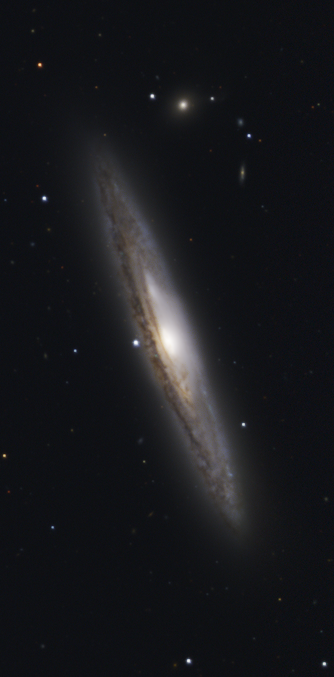
\includegraphics[width=0.49\textwidth]{../Images/chapter_1/SN2024gy_pre-SN.png}
    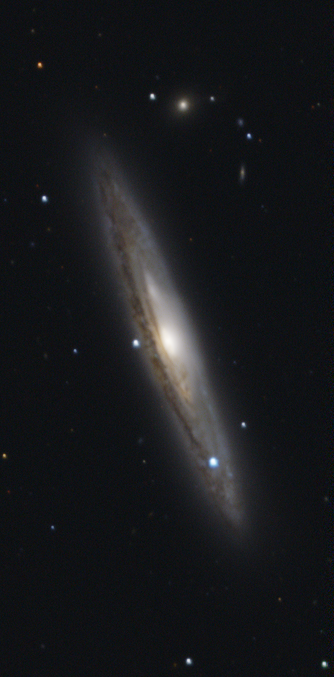
\includegraphics[width=0.49\textwidth]{../Images/chapter_1/SN2024gy_active.png}
    \caption{\ztfg\ztfr\ztfi\ composite image of NGC 4216 using observations taken by ZTF.\\
    \textbf{Left:} composite image of observations taken before 1 January 2024.\\
    \textbf{Right:} composite image of observations taken between 5 and 19 January 2024, the first two weeks after the first detection of the Type Ia SN~2024gy. (Credit: Benjamin Nobre Hauptmann)} %30, 29, 14 (gri SN images) & 35, 31, 30 (gri pre-SN images) given to Benjamin, subset used based on data quality, exact numbers not so relevant
    \label{2024gy_ZTF}
\end{figure}


\subsection{Core-collapse SNe}
\label{CCSN}
As was mentioned at the end of section \ref{ge_8_Msol}, stars above 8 $M_\odot$ end their lives in a CCSN when the core implodes into a compact object due to the effects of gravity. The outer layers fall in as well but bounce back outwards as the enormous amounts of released gravitational energy from the collapsing core is imparted on the outer layers, heating them up and expelling them outwards at high velocities. The light coming from the cooling of this material and the radioactive decay of newly formed unstable nuclei into stable ones cause the SN to rise rapidly in brightness. Within hours after the explosion it is bright enough to be observed in other galaxies, peaking after several days to weeks at an absolute magnitude in the range of -16.5 mag to -18.5 mag depending on the type of CCSN \citep{SN_M_dist}. This is what we observe as the SN event, and by analysing their spectra around peak light they can be classified based on the visible elemental emission and absorption lines.

The composition of the outer layers of the progenitor depends heavily on the life of the star. Most CCSNe have hydrogen in their envelope, which will show up in the SN spectra as strong Balmer P Cygni profiles. These are known as Type II SNe. Photometric features of the light curve (the SN brightness as it changes over time) are also used in SN identification, leading to subtypes such as SN IIL or SN IIP for Type II SNe that show a linear decline or a plateau, respectively. High mass-loss rates, due to a high stellar wind \citep{He-star_pre_SN_evol_mass_loss} or the presence of a binary companion \citep{He-star_pre_SN_evol_binaries}, can however strip the hydrogen layer, leaving the helium shell as the outermost part of the progenitor at the moment of explosion. When there is no hydrogen visible in the spectrum, the SN is of Type I. CCSNe that show no H lines but do have He lines in their spectra are called Type Ib SNe. In some extreme cases even the helium layer has been stripped away, resulting in SNe without H or He lines in their spectra, known as Type Ic SNe. Transitional objects, where a layer is mostly but not completely stripped, are also known \citep{SN_large_pic}.\\

Photometric classification is cheaper as photometry is easier to obtain, but it cannot differentiate between subtypes that are defined on the presence, strength, or absence of specific elemental lines, leading to broader classifications with less certainty. Besides this, many of the differences that make certain SNe interesting are visible at early times, while a SN needs to evolve up to a certain point to have a light curve that can be used for classification. For these reasons, a common strategy is to use dedicated large-scale surveys such as the ZTF to find new SNe within days after explosion using photometry, and using different telescopes to follow these up with spectroscopy for classification.

\subsection{Thermonuclear SNe}
\label{SNIa}
Besides CCSNe are the more commonly observed thermonuclear SNe (Type Ia SNe, SNe Ia), which are exploding WDs after fusion in their core has been ignited through some mechanism (see section \ref{Ia_progenitors}). The more massive the WD, the easier it is to ignite as the nuclei are forced closer together. Since the WD is degenerate, the energy released by a single fusion event can completely be used to heat up the surrounding material and let it fuse as well, leading to a runaway process where the entire WD tries to fuse to iron-peak elements on a timescale of seconds. This process disrupts the entire star, expelling the material outward at relativistic speeds \citep{Ia_thermonuclear}. While not all material in the WD is fused, most of the mass ends up in $\Nififtysix$, with typical SNe Ia producing between 0.3 -- 0.8 $M_\odot$ of $\Nififtysix$ \citep{Ia_Ni56_yield}. This is an unstable nucleus and decays as
\begin{equation}
    \Nififtysix\ \xrightarrow{6.1\text{ d}}\ \Cofiftysix\ \xrightarrow{77.3\text{ d}}\ \Fefiftysix,
\end{equation}
with $\Fefiftysix$ being the stable end product of the decay chain. The key spectral signatures of a SN Ia are the absence of hydrogen lines and broad \SiII\ absorption features in their spectra around peak brightness. At first, the ejecta are dense and opaque, and only photons from the outer layers can escape. As the ejecta expand, they become more transparent, and the slower moving inner layers become visible as the photosphere recedes inwards through the layers. Therefore, by taking spectra at different phases, a map of the elemental abundances in velocity space can be built. As different models of the progenitor system and explosion mechanisms predict different compositions, this is a popular way to compare models to observations \citep[e.g.][]{ptf11kx,de_2019_18byg,2020sck_Iax,2021rhu}.

The SN reaches peak brightness around three weeks after the explosion and starts to fade again. The main power source that governs the rate at which the SN fades is the decaying $\Nififtysix$, resulting in a linear decline of the light curve in magnitude space. In the near-infrared there is a second peak a few weeks after the first, which is suggested to be the result of a decrease in opacity due to the changing ionization state of iron group elements \citep{2nd_max}. Figure \ref{Ia-norm_example} shows an example of a well-observed normal SN Ia.

\begin{figure}
    \centering
    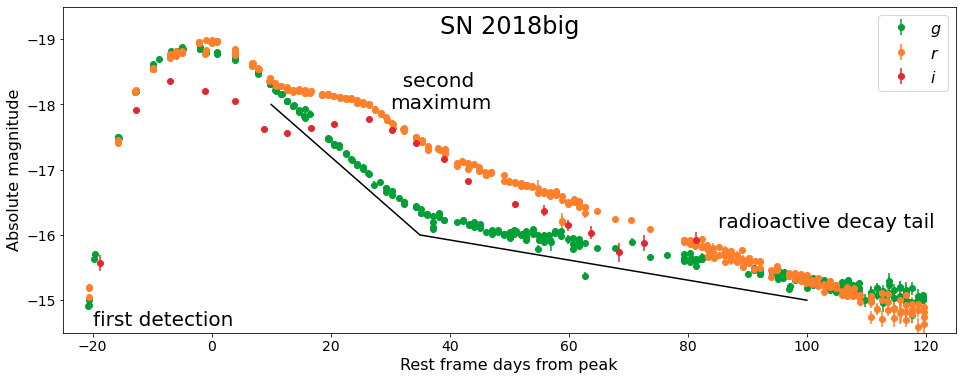
\includegraphics[width=\textwidth]{../Images/chapter_1/Ia-norm_example.png}
    \caption{ZTF \ztfg\ztfr\ztfi\ light curve of a SN Ia in the rest frame and absolute magnitude, corrected for Milky Way extinction but not for host extinction. The \ztfg-band clearly shows a change in the decline rate as $\Cofiftysix$ decay becomes dominant over $\Nififtysix$ decay (as shown by the broken black line). The \ztfr- and \ztfi-band show the second peak.}
    \label{Ia-norm_example}
\end{figure}

\subsubsection{Standardizable candles}
\label{Standard_candle}
Most SNe Ia peak around an absolute magnitude of -19.5 mag, making them brighter than CCSNe. Some SNe Ia become brighter than others, but they also evolve slower. This is called the Phillips relation \citep{phillips_rel}, and it can be used to infer the absolute peak brightness based on how fast it evolves. \citet{Tripp_colour_rel} improved the standardization by adding a second term: the so-called colour luminosity term. This accounts for the intrinsic SNe Ia colour, as bluer SNe Ia are brighter. These days a third term is included, which accounts for environmental dependencies and is implemented as a step function \citep{Kelly_mass_step, Sullivan_mass_step}. The resulting standardization formula is given by
\begin{equation}
    \mu_\text{obs} = m_B - M_0 + \alpha x_1 - \beta c - \gamma p,
\end{equation}
where $\mu_\text{obs}$ is the observed distance modulus. $m_B$ and $M_0$ are the apparent and absolute B-band magnitude, respectively. $x_1$ is the SN stretch, $c$ its colour, and $\alpha$ and $\beta$ are the coefficients used to correct for these effects. $\gamma$ is the size of the step function, and $p$ determines when this step needs to be applied.

Using the standardisable nature of SNe Ia allows their distance to be measured, as well as the distance between Earth and the host galaxies they reside in. At the same time, the redshift of the host galaxy can be measured from the spectra. With these values together, the Hubble constant $H_0$, which measures the expansion rate of the universe, can be measured. The SH0ES team \citep{SH0ES} used the Pantheon+ sample \citep{Pantheon+} to measure the expansion rate of the universe and found it to be $H_0 = 73.30 \pm 1.04$ km s$^{-1}$ Mpc$^{-1}$.


\subsection{Other types of transients}
\label{Other_trans}
There are other types of transients besides the SNe mentioned above. Some SNe become much brighter than normal events and are therefore called superluminous SNe (SLSNe). Supermassive black holes (SMBHs) in the centre of galaxies can cause a variety of transient events such as tidal disruption events (TDEs) or ambiguous nuclear transients (ANTs), or a galaxy could have an active galactic nucleus (AGN). Some types of stars also pulsate, and vary in brightness over time. All of these can show up as transients in surveys looking for changes in the night sky on a day-to-day basis.


\subsubsection{SLSN - Superluminous Supernova}
SLSNe are SNe that have a higher peak luminosity than normal SNe, in some cases reaching over 5 magnitudes brighter than normal events at their peak \citep{SLSN_Gal-Yam}. Like normal SNe, they can be classified into Type I and Type II based on the absence or presence of hydrogen emission lines in their spectra. One of the main puzzles regarding these types of events is the source that powers their superluminous nature. Different types of models have been put forward, using magnetars \citep{Maeda_SLSN_magentar}, black holes \citep{SLSN_BH}, radioactivity \citep{Kasen_SLSN_pair_instab}, or interaction with circumstellar material (CSM) \citep{Late-time_CSM_SLSNE_I} to push the brightness significantly above that of regular SNe. Each of these has different strengths and weaknesses.


\subsubsection{AGN - Active Galactic Nucleus}
An AGN is the central region of a galaxy in which a SMBH accretes matter at a high rate, releasing a part of the potential energy as heat and radiation. As a result of this, the AGN has a very high luminosity compared to the rest of the galaxy, with different orientations of the system resulting in different types of AGN \citep{Antonucci_1993_AGN, Urry_1995_AGN}. As the stream of matter being accreted is inhomogeneous, the accretion rate and luminosity change over time. In some cases AGN variability is so extreme that it changes the entire spectrum of the AGN, with (dis)appearing broad emission lines and continuum flux. These are so-called changing-look AGN (CL-AGN) \citep[see][for a review]{CLAGN}. AGN variability can be used to estimate the SMBH mass through reverberation mapping \citep{Reverberation_mapping, Reverberation_Peterson}. Fast moving clouds close to the AGN change the strength of line emission based on how strongly they are illuminated by the AGN. The delay between a luminosity change in the AGN continuum and the broad emission line features coming from these clouds gives a measure of their distance, while the width of the emission lines gives a measure of their velocity. From these measurements the SMBH mass can be estimated using Kepler's third law.


\subsubsection{TDE - Tidal Disruption Event}
In some cases a star can get too close to the SMBH and get tidally disrupted \citep{Rees_1988_TDE, Strubbe_2009_TDE}. In a TDE the star gets ripped apart due to the strong gravity of the SMBH and forms an accretion disk of hot gas that gets accreted onto the SMBH. The distance at which the TDE occurs depends largely on the SMBH mass, and for SMBHs more massive than $\sim10^8 M_\odot$ the tidal disruption radius lies within the event horizon, meaning that TDEs cannot be observed around the most massive SMBHs \citep{Hills_mass}. The other dependency of the tidal radius is the difficulty to disrupt a star. Compact objects such as WDs are very difficult to disrupt and thus have a smaller tidal radius. A red giant, on the other hand, has outer layers that are very loosely bound to the star, and the star is therefore easier to disrupt at a larger radius, though this might also result in a partial tidal disruption where only the outer layers are stripped while the stellar core survives the encounter. TDEs can become brighter than SNe, with the brightest event ever observed being AT 2021lwx (ZTF20abrbeie, nicknamed "Scary Barbie"), which is thought to be the disruption and accretion of a giant molecular cloud \citep{Scary_Barbie, 2021lwx_Wiseman}.


\subsubsection{ANT - Ambiguous Nuclear Transient}
Some nuclear variability does not quite fit the known classes of AGN or tidal TDEs, showing characteristics of both types of events. These events have been named ambiguous nuclear transients \citep[ANTS;][]{Kankare_ANT, 2020ohl_Hinkle, Hinkle_MIR_ANT_echo, Hinkle_Extreme_nuclear_transients/ANTs, wiseman_ztfants} and rise up quickly, reaching peak brightness within a few weeks before declining very slowly over hundreds of days, although their decline rates are variable.


\subsubsection{Variable stars}
Some stars show variability as well, with the brightness of certain types of stars oscillating by a magnitude or more. The most famous class of variables are Cepheids, whose regular oscillation period of the order of days is related to their absolute magnitude. They are bright enough to be visible in nearby galaxies, which makes them useful to calibrate SN Ia distance measurements when building the distance ladder \citep{Cepheids_Gibson, Cepheids_Saha}. Other types of stars, such as Mira variables, are much more extreme in their change of brightness and have periods $>100$ days \citep{Mira_varibs}.


\section{SN Ia subclasses}
As has been stated in section \ref{Standard_candle}, most SNe Ia explosions evolve in a very similar way with a tight relation between their peak, colour, and rate at which they evolve. These are called normal SNe Ia, or SNe Ia-norm. This name suggests the existence of abnormal SNe Ia besides the normal ones. This is indeed the case, in fact there is an entire zoo of subclasses that have photometric and/or spectroscopic differences from SNe Ia-norm. \citet{Taubenberger_plot} showed the different subclasses of SNe Ia together by plotting their peak absolute B-band brightness as a function of $\Delta m_{15}$(B), which is the difference in brightness in the B-band between the SN at peak brightness and 15 days after the peak in the SN rest frame expressed in magnitudes. This plot is also shown in Fig.~\ref{Taub_plot}.

\begin{figure}
    \centering
    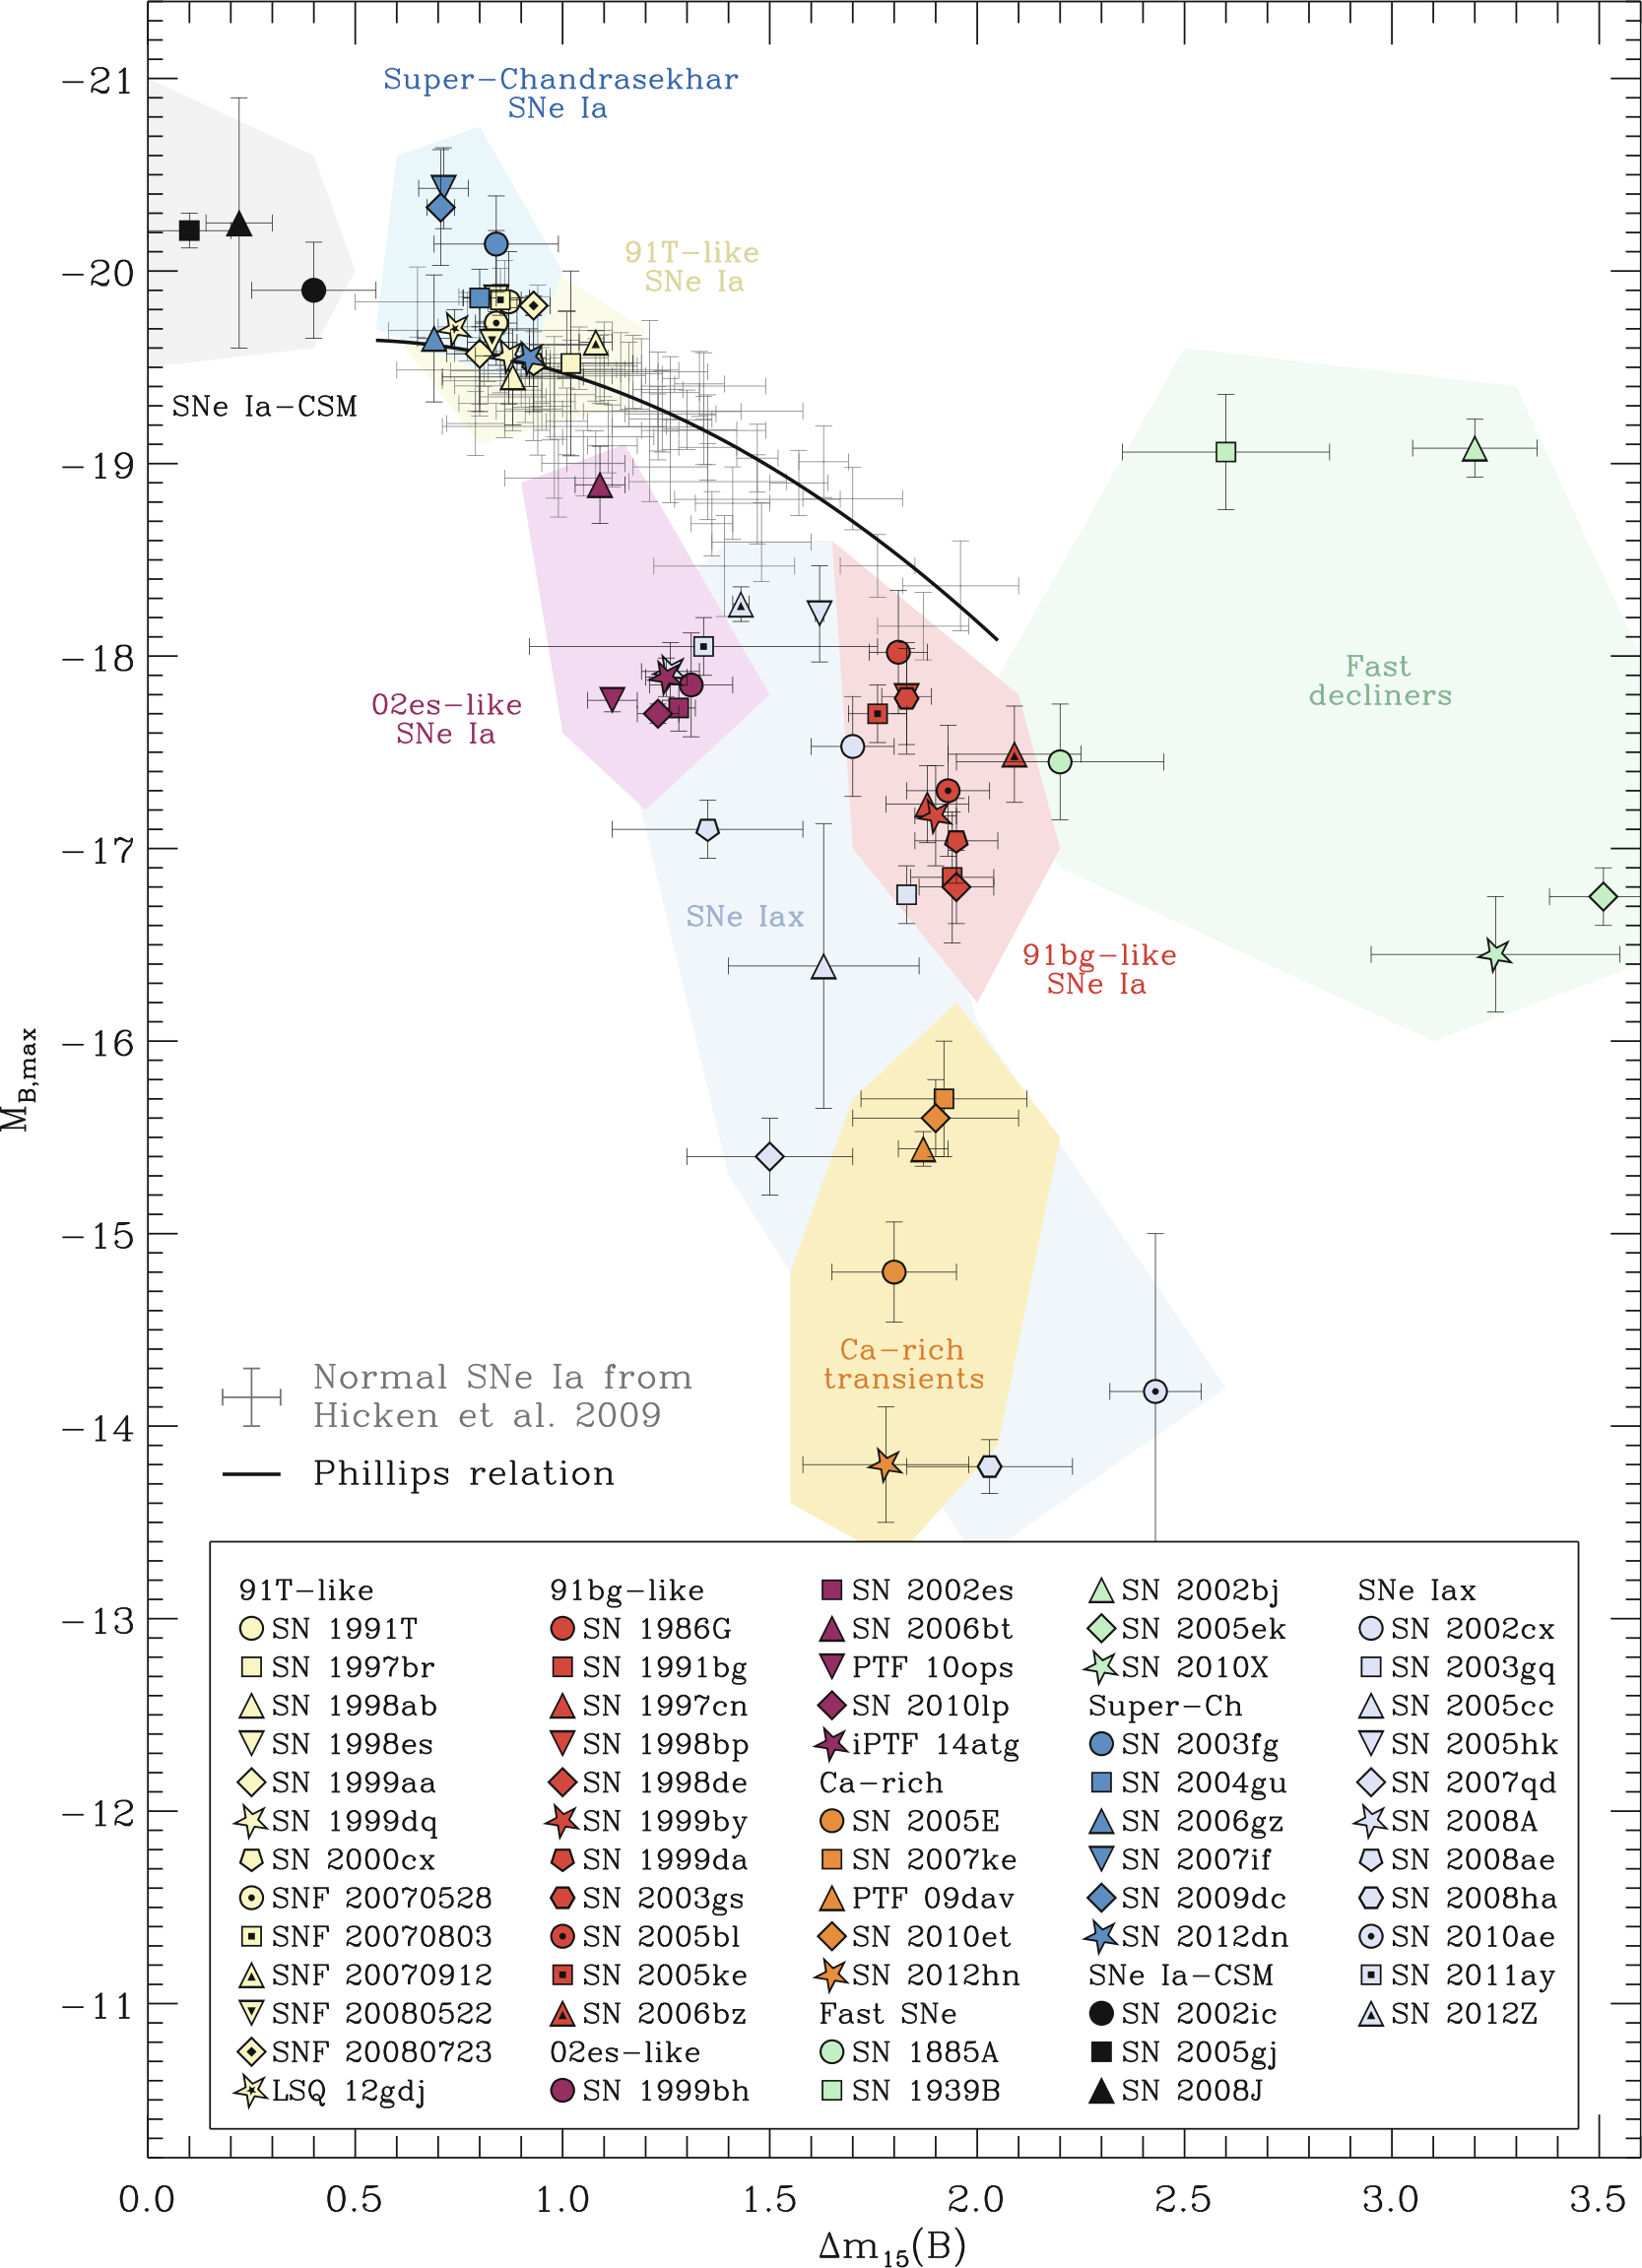
\includegraphics[width=\textwidth]{../Images/chapter_1/Taub_plot.png}
    \caption{Subclasses of SNe Ia. The peak absolute B-band magnitude is plotted as a function of $\Delta m_{15}$ in the same band. Normal SNe Ia lie along the Phillips relation, which is shown with a black line. Most of the non-normal subclasses can be separated from normal SNe Ia based on these two values alone. The main exception are the 91T-like SNe, which form a subclass based on their spectral differences from normal SNe Ia. This figure was taken from \citet{Taubenberger_plot}.}
    \label{Taub_plot}
\end{figure}

Recently, \citet{DR2_diversity} made a similar plot but in the \ztfg-band, using the carefully curated sample of SNe Ia from the Zwicky Transient Facility's second data release \citep[ZTF SN Ia DR2,][Smith et al., in prep.]{DR2_Overview}. They show that $\sim75$\% of all SNe Ia are normal events that can be standardized and used for distance measurements. After that, the two largest subclasses are the SNe Ia-91T ($\sim12$\%) and SNe Ia-91bg ($\sim6$\%), leaving $\sim7$\% as the combined total of various other subclasses.

Different subclasses have a preference for different environments. By studying these, the characteristic properties of their light, and the connection to their environments, we can learn more about the properties of their progenitor systems and the exact mechanisms that are involved in SN Ia explosions.


\subsection{Photometric differences}
The Phillips relation is easily visible in Fig.~\ref{Taub_plot}, and SNe Ia-norm lie in a narrow strip around it. Most subclasses can be distinguished from SNe Ia-norm by photometry alone. The (aptly named) fast decliners fade unusually quickly after reaching peak brightness, while SNe Ia-CSM barely fade at all in the first few weeks after reaching their peak brightness. SNe Iax never reach the peak brightness of a normal SN Ia, which in some models is explained through the explosion failing to fully disrupt the WD \citep{Iax_model_1, Iax_model_2}. Super-Chandrasekhar SNe Ia on the other hand are brighter than what would be expected from a $M_\text{Ch}$ WD explosion. Many subclasses are named after a prototypical SN that defines the subclass.


\subsection{Spectroscopic differences}
Besides photometric differences, most subclasses are also spectroscopically different from SNe Ia-norm. Some have stronger emission lines of particular elements, others have weaker ones. Ca-rich transients \citep[e.g.][]{Ca-rich_2010, Ca_rich_2012, Ca-rich_rate} show \CaII\ emission lines in their nebular spectra that are much stronger than for other SN Ia types. The spectra of super-Chandrasekhar SNe show that their ejecta move considerably slower compared to other subclasses, which, together with their high luminosity, is consistent with a double degenerate merger scenario \citep{2003fg_SuperCh, 06gz_SuperCh, 09dc_SuperCh}.

The SN Ia-91T subclass lies at the bright end of the Phillips relation, and thus cannot be identified photometrically but can therefore be normalized and used for distance measurements. Spectroscopy however reveals that this subclass evolves differently as it rises towards peak brightness, showing a blue pseudo-continuum with two strong \FeIII\ absorption multiplets instead of intermediate-mass element lines. They also have a preference for younger stellar populations \citep{Filippenko_91t, 91T}, although this preference is not seen in \citet{DR2_diversity}.


\section{SN Ia progenitor systems}
\label{Ia_progenitors}
WDs are stable objects on their own, but they can be made to explode under certain circumstances. Not all stars are single, and WDs in a binary system can interact with the other star and start accreting matter coming from the so-called donor star. As the radius of a WD is inversely proportional to its mass (Equation \ref{nonrel_WD_eq}), it will shrink as it becomes more massive until the point is reached where fusion is ignited in the core of the WD, triggering its explosion.

Assuming that the stars have been in the binary system since formation, and since more massive stars have a shorter lifespan, the more massive star has turned into the WD. Therefore, the donor has to be $<8$ $M_\odot$ (though due to stellar and especially binary evolution the mass of the donor has likely changed since formation). The donor could still be burning hydrogen or have evolved to the later stages in its life, up to and including becoming a WD as well. The many possibilities for the donor star is called the progenitor problem, which is currently still being debated. Different progenitor scenarios can broadly be put into one of two categories based on whether the donor star is a compact object (double degenerate) or not (single degenerate). Artistic impressions of these two scenarios are shown in Fig.~\ref{single_double_deg_mods}.

\begin{figure}
    \centering
    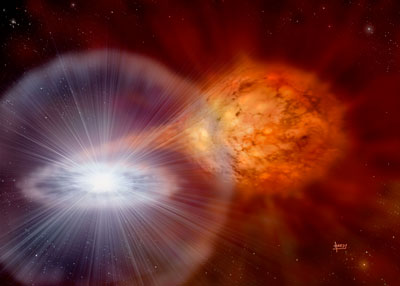
\includegraphics[height=0.229\textheight]{../Images/chapter_1/single_deg.jpeg}
    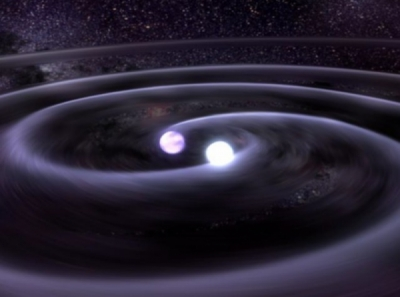
\includegraphics[height=0.229\textheight]{../Images/chapter_1/double_deg.jpeg}
    \caption{\textbf{Left:} Artistic impression of a single degenerate system, where the white dwarf accretes material coming from the surface of the donor star. Image credit: STFC / David Hardy. \textbf{Right:} Artistic impression of a double degenerate system where two white dwarfs spiral in to each other while releasing gravitational waves. Image credit: NASA / Tod Strohmayer (GSFC) / Dana Berry (Chandra X-Ray Observatory).}
    \label{single_double_deg_mods}
\end{figure}


\subsection{Single degenerate}
The most straightforward and classical way to explode a WD is by adding mass to a near-$M_\text{Ch}$ WD until carbon is ignited in the core due to compressional heating. The companion star fills its Roche lobe, and material from the outer layers is syphoned onto the WD. The donor can fill its Roche lobe while it is still a main sequence star, when it has evolved into a red giant, or it may even be a helium star whose hydrogen layer has been stripped due to binary interactions \citep{Whelan_classical_Ia_mod, Nomoto_single_degenerate}. In delayed-detonation models the WD first expands during a deflagration phase, which then transitions into a detonation after the WD becomes unbound \citep{Kholov_Del_det, Mazzali_common_mechanism}.

It is also possible that the WD and red giant companion enter a common envelope phase. The WD merges with the hot core of the red giant, forming a rapidly rotating, WD-like degenerate core with $M_\text{core}>M_\text{Ch}$ inside the red giant. The angular momentum prevents the core from collapsing in on itself but it is gradually lost until it can no longer support itself, triggering the SN Ia explosion in the so-called core degenerate scenario \citep{Kashi_core_deg}.


\subsection{Double degenerate}
If both objects are WDs, the primary (more massive) WD can still accrete material from the secondary WD in a stable Roche lobe overflow scenario \citep{CO_accretion_II, CO_accretion_I}. In non-classical models, a sub-$M_\text{Ch}$ WD can explode by first slowly accreting and building up a layer of helium on its surface, which explodes after a sufficient amount of material is gathered. As this explosion wraps around the outside of the WD, it sends a shockwave into the interior of the star, which culminates near the centre and temporarily increases the local pressure. If this is enough to ignite carbon fusion, the second detonation is triggered, which disrupts the star and results in the main SN \citep{Taam_ddet, Livne_ddet, Shen_ddet, Fink_ddet}.\\

In other scenarios the WDs fully merge, either dynamically or violently. In the dynamical scenario the WDs lose angular momentum as it is radiated away through gravitational waves \citep{Iben_Double_degenerate, Webbink_Double_degenerate}. An artist's impression of this scenario is given on the right side of Fig.~\ref{single_double_deg_mods}. As the WDs come closer, the less massive companion fills its Roche lobe, and material starts flowing onto the primary. As the companion loses mass, its radius increases, leading to more mass loss until the entire star is disrupted. Around half of the material forms a disk around the surviving WD while the rest falls directly onto its surface. Very little material is expected to be flung out of the system. As the system evolves, it eventually explodes in a SN Ia.

In collisions or violent mergers of two WDs a detonation can occur during the merger at the location of the accretion stream due to its high density and temperature \citep{Rosswog_merger, Pakmor_merger, Pakmor_merger2}. This might either directly start carbon fusion at the ignition site or cause a surface explosion that again wraps around the WD and compresses its interior causing a second ignition, depending on the system and WD masses. The asymmetry of this system when it explodes is expected to cause significant asymmetry in the ejecta and its composition in different directions. This is expected to lead to different amounts of polarization of the SN light, depending on the angle between the plane of rotation and the line of sight \citep{Wang_merger_pol, Bulla_merger_pol}.


\section{SNe with circumstellar material}
The progenitor system of a SN is not completely isolated. Through mechanisms such as high stellar winds or binary interaction, a significant amount of material can end up close to the explosion site before the explosion occurs. This is called circumstellar material (CSM), and since it usually originated from the progenitor system, CSM can give new insights into the history of the progenitor system and the sequence of events that led it to explode.\\

Ejecta from the SN explosion are expelled at high velocities and quickly catch up with the much slower moving CSM. As the ejecta slam into the CSM, shockwaves are produced and energy is deposited into the CSM, which starts to emit light of its own. This new light source alters the light curve, making it brighter and slowing or even stalling its decline. CSM interaction also shows up in the spectra as emerging narrow emission lines that give clues about the composition of the slower moving material. Eventually the ejecta overtake the CSM and its signal fades as the CSM is swept up.

Another way in which the presence of CSM has been inferred is through the presence of narrow, time-varying absorption lines, indicating that they evolve alongside the SN \citep[e.g.,][]{2006X, Sternberg_NaID}. However, these absorption lines are not always seen, and their behaviour varies from object to object, making it difficult to interpret them consistently. Light echoes can also provide an opportunity to study circumstellar and interstellar material, though the difficulty to geometrically separate them from the SN location and their weak nature makes this only possible for SNe in the Milky Way or nearby galaxies \citep{Patat_light_echoes, Tycho_Brahe_classif, 2012cg}.

\begin{figure}
    \centering
    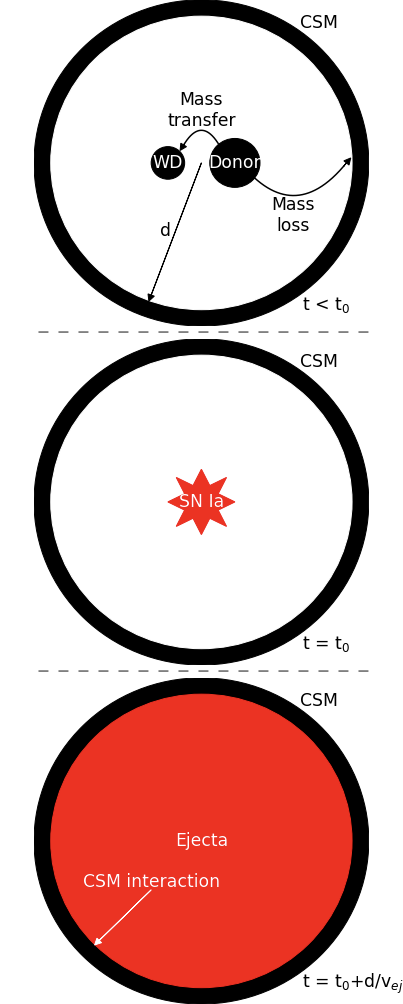
\includegraphics[height=0.847\textheight]{../Images/chapter_1/CSM_sketch_vert.png}
    \caption{Schematic view of a SN Ia-CSM event. \textbf{Top:} The progenitor system containing a WD feeding on material from the donor star. Through various mechanisms a fraction of this material can be lost from the system and end up as CSM in a disk or shell at a distance $d$ around the progenitor system. \textbf{Middle:} The WD explodes as a SN Ia. This can be a SN Ia-norm or a peculiar object, depending on the progenitor system. The ejecta start travelling outwards from the explosion site. \textbf{Bottom:} The ejecta catch up to the CSM and start interacting with it, causing the CSM to start emitting light as well as it is swept up. This results in a slowing down of the photometric light curve decline and the emergence of narrow emission lines in the spectra.}
    \label{Ia-CSM_mod}
\end{figure}

CSM can be created by different mechanisms depending on the progenitor system, and its composition depends on the type of donor star present. In the single degenerate scenario, CSM rich in hydrogen can be created by a WD generating a fast wind, blowing away a part of the material it received from the mass transfer \citep{single_degen_CSM_gen}. In the double-degenerate scenario, part of the tidally disrupted secondary WD becomes unbound from the system, creating (H-poor) CSM and may be able to produce detectable signatures depending on the time between the tidal disruption and the SN Ia explosion \citep{Double_degen_CSM_gen}. The core degenerate scenario could provide a massive amount of hydrogen-rich material near the explosion site \citep[e.g. for SN 2014J,][]{2014J_core_deg}, though the signatures of this scenario could be ambiguous with interacting SNe IIn, leading to confusion \citep{Inserra_2016}. \citet{snips} proposed that the core degenerate and double degenerate scenarios could lead to SNe Ia exploding inside planetary nebulae, possibly resulting in observable time-varying \NaID\ absorption lines or CSM interaction.

Figure \ref{Ia-CSM_mod} shows a schematic view of the creation of a CSM shell (or ring depending on how mass is lost from the SN Ia progenitor system) and the subsequent interaction between the CSM and SN ejecta. When the SN explodes the ejecta will initially expand within the gap between the progenitor system and the CSM, and its spectrum will look like that of a non-interacting class of SN Ia that may or may not display absorption features caused by the CSM if it is in the line of sight. Compared to the ejecta, which are travelling at $v_\text{ej}$, the CSM is practically stationary but at a distance $d$ from the explosion site. This means that the ejecta need a time $t=d/v_{ej}$ to reach the CSM and start to interact with it. Only then does the event transform into a SN Ia-CSM with new narrow emission lines. This later transformation explains why in some cases objects are reclassified as Ia-CSM after first being classified as something else (e.g. SN 2020aekp, which was first classified as a SN Ia by \citealt{2020aekp_1st_classif} but reclassified as a SN Ia-CSM by \citealt{2020aekp_reclassif}).


\subsection{The SN Ia-CSM subclass}
\label{Ia_CSM}
SNe Ia-02ic, also known as SNe Ia-CSM, are the subclass of thermonuclear explosions that show signs of CSM interaction. This often shows up as a peculiar long-lived light curve along with narrow Balmer emission lines, which is a clear indicator of this signal coming from CSM as SNe Ia are expected to be hydrogen-poor. The prototypical event, SN 2002ic, showed narrow \Halpha\ and \Hbeta\ lines, and the slowly declining light curve was found to be consistent with $\sim1.3$ $M_\odot$ of CSM \citep{02ic_H_det, Hamuy_02ic, 02ic_slow_decay, single_degen_CSM_gen}.

Currently, there are several dozen known SNe Ia-CSM \citep{2005gj, Ia-CSM_Silverman, Ia-CSM_BTS}. In all cases the interaction started within two months after the explosion, leading to their (re-)classification after spectroscopic confirmation. The amount and duration of interaction varies quite significantly from one object to another. While some members such as SN 2018gkx and SN 2020xtq mainly feature an unusually slow decline rate, other objects such as SN 2020aekp have a plateau for several 100 days before starting to fade away slowly \citep{Ia-CSM_BTS}.

SN 2011km (PTF11kx) is a well-observed SN Ia-CSM event that shows signs of a complex CSM consisting of multiple shells with which the SN ejecta interact. \citet{ptf11kx} show that its photometry is similar to 91T-like objects before the CSM interaction begins, and explain SN 2011km using a symbiotic nova progenitor system. \citet{Ia-CSM_and_91T_connection} also suggested a link between SNe Ia-91T and SNe Ia-CSM as they show similarities in their peak brightness and spectroscopy before the start of the interaction. In some cases, a 91T-like SN could start interacting with CSM hundreds of years after the explosion, as has been suggested for Kepler’s SN \citet{Kepler_91T, Kepler_CSM}.

Another interesting SN Ia-CSM is SN 2020eyj, which \citet{Kool_He_CSM} present as the first detection of a SN Ia-CSM interacting with He-rich material. Up until then all members of the subclass had shown strong \Halpha\ emission and weak He signatures. SN 2020eyj, however, showed little to no H present in the CSM. This suggests that the progenitor system contained a He star. This was also the first time a SN Ia was detected in the radio. Non-detections in normal SNe Ia suggest a clean environment for the ejecta to expand in, while in this case there is a lot of material present.


\subsection{CSM in CCSNe}
Some CCSNe show interaction with CSM as well. The events are subclassified as SNe~IIn, SNe Ibn, or SNe Icn, with the `n' for narrow emission lines. As stated in section \ref{CCSN}, the difference between these three main types of SNe is the amount of material that has been stripped prior to explosion. Mass can be lost through binary interaction stripping away the outer layers of the star prior to explosion \citep{Ic_binary_progenitors}. Massive stars have also been known to have strong stellar outflows and winds. The existence of Wolf-Rayet stars shows that very massive stars can lose their entire hydrogen envelope, and they are thought to be one of the very last stages in the life of the star before it explodes in a SN Ib or SN Ic \citep{WR_as_progenitors, 2019hgp}. Current models prefer the binary scenario due to the low amount of confirmed disappearances of progenitor stars \citep{CCSN_disappeared_progenitor}.

The CSM often resides close to the progenitor and can be thick enough to obscure features of the underlying SN, depending on the geometry and orientation of the system \citep{1994W, PTF11iqb}. The short distance between the SN and CSM suggests that the material was ejected recently, and in some cases precursor events have been observed prior to the final SN explosion (e.g. SN 2011ht, \citealt{2011ht} and SN 2020pvb, \citealt{2020pvb}). CSM residing close to the progenitor causes most interacting CCSNe to show signs of CSM interaction almost immediately after the explosion. However, examples of the interaction starting much later have been found as well, suggesting that their CSM has been ejected a long time ago \citep{2008iy, late-CSM_IIn_Spitzer}.

Recently, SN 2021yfj was discovered to be a new type of SN and given the classification of SN Ien \citep{Ien_class}. This object showed highly ionized silicon, sulphur, and argon lines but barely any carbon, oxygen, helium, or hydrogen. This suggests the progenitor was a massive star stripped all the way down to its final layer before the iron core. The classification leaves space for the yet-to-be-discovered explosion of a slightly less stripped star in a SN Type Idn, which would have no carbon but strong oxygen, neon, and magnesium emission lines, as well as their non-interacting counterparts and transitional objects. \citep{Ien_disc}.\\


\subsection{Distant CSM}
As stated in section \ref{Ia_CSM} and shown in Fig.~\ref{Ia-CSM_mod}, there is a delay between the SN explosion and the start of CSM interaction due to the distance between the progenitor system and CSM. All objects that are currently classified as SNe Ia-CSM on the Transient Name Server (TNS)\,\footnote{\url{https://www.wis-tns.org/}} have shown signs of interaction at or around peak brightness. Assuming an ejecta velocity of $v_\text{ej} \sim 20\,000$ km s$^{-1}$ and that the interaction starts on average around the SN peak $\sim3$ weeks after the explosion, the CSM is located at a distance $d\sim3.5\times10^{15}$ cm of the progenitor system \citep{Ia-CSM_BTS}. If however the CSM is at a distance of $d\sim10^{17}$ cm, ejecta with the same $v_\text{ej}$ would need $\sim1.5$ years to catch up and start interacting.

In the effort to systematically search for such late-time CSM interaction, \citet{2015cp} looked at old ($\geq1$ year) SNe using the \textit{Hubble Space Telescope} (HST). They focused their search on subclasses that are associated with CSM interaction, such as SNe Ia-91T \citep{Ia-CSM_and_91T_connection}. Out of 72 targets, only ASASSN-15og and SN 2015cp were found to show late-time CSM interaction. ASASSN-15og is a SN IIn with detected CSM interaction around its peak, and was used as a control object. SN 2015cp has been classified as a SN Ia-91T without signs of CSM interaction around its peak. This showed that late-time CSM interaction may be systematically missed due to SNe~Ia not being actively followed at these phases. From a progenitor point of view, this means that material can be ejected from the system prior to the explosion, giving it time to travel further before being caught up by the SN ejecta.

\citet{GALEX_Late_CSM} used archival UV-band data from the \textit{Galactic Evolution Explorer} (GALEX) to look for late-time CSM interaction in SNe Ia. Out of a sample of 1080 SNe Ia, 4 were detected in the UV near peak, but none showed signs of late-time CSM interaction. They show that this type of CSM interaction is rare, occurring between 500 to $1\,000$ d after the initial discovery of the SN in $<5$\% of the SNe Ia at a strength similar to SN 2015cp, and a decreasing percentage as the interaction gets stronger.


\section{In this thesis:...}
In this thesis I will present my work on the search for signs of late-time interaction in SNe Ia using observations taken by ZTF. CSM is connected to the mass loss history of the progenitor system, and more distant CSM has been ejected a longer time ago. By studying late-time CSM it is possible to learn more about the mass loss history of the progenitor system, and it can hold clues to the type of progenitor scenario that the system belonged to.\\

In chapter \ref{chap:obs} I will introduce ZTF as well as the other facilities that have been used to gather data that is presented in this thesis. I will also give an overview of the basics of observing, some of the types of data that can be obtained, and the basic steps that are required to reduce them to something that can be used in further analysis.

Chapter \ref{chap:DR2_search} is an adaptation of \cite{Terwel_2024_paper1}, and presents my search for late-time signals in the ZTF SN Ia DR2, which consists of $3\,628$ spectroscopically classified SN Ia that were first discovered between March 2018 and October 2020. It also details the pipeline and analysis tools I developed to search in a consistent manner (Section \ref{DR2_analysis}).

It might be possible that a late-time signal is observed by ZTF while the main transient occurred before the survey started. In chapter \ref{chap:pre-ZTF_search} I search for this type of event using a slightly modified version of the pipeline used for the DR2 search. As the analysis is exactly the same whether the original transient was a SN Ia, SN II, or any other type of transient, I search through a sample of 8707 transients that were first discovered between 1 January 2008 and 1 January 2018.

Up to this point my search has been through archival data only, with the obvious drawback that it is very likely that any recovered late-time signal cannot be followed up on. By further modifying the pipeline, I search in chapter \ref{chap:Real-time} for late-time signals in SNe Ia in real-time using the latest ZTF observations with the goal to follow up photometrically and/or spectroscopically using other telescopes.

Finally, in chapter \ref{chap:Conc_and_fut} I conclude on the results of searching through these three samples and finish with possible continuations of this search, modifications, and possible alternative usages for this or a similar pipeline.

To convert between apparent and absolute magnitude I assume a flat $\Lambda$CDM cosmology with H$_0 = 67.7$ km s$^{-1}$ Mpc$^{-1}$ and $\Omega_\text{m} = 0.310$ \citep{Planck18VI} throughout this thesis.

\end{document}
%!TEX root = ../main.tex
\documentclass[a4paper,oneside,12pt, class=Latex/Classes/PhDthesisPSnPDF, crop=false]{standalone}
\usepackage{setspace}
\begin{document}
\doublespacing
\chapter{Observing in the optical regime}
\label{chap:obs}

\color{red}To do list: Add refs, sometimes slightly confused which tense to use, recheck carefully, opmaak, reference about the LP light pollution restriction laws? mention gain (e$^-$ / ADU conversion) and read noise (mean e$^-$ added per pixel at readout) as well somewhere. \color{black}

Astrophysicists face the challenge of not being able to set up and control their experiments. The universe is our laboratory but all we can do is see or detect the results while often not knowing the exact setup of the experiment. Models are made to explain and predict the behaviour of planets, stars, galaxies, etc. but ultimately observations are needed to compare against and test our models. My work relies heavily on observational data, and in this chapter I will introduce the different types of observations that are used throughout this thesis (section~\ref{observation_types}), telescopes and instruments that are used to obtain these observations (section~\ref{telescopes}), and a quick overview of how to calibrate the raw images and extract useful data (sections~\ref{calibration} and~\ref{reduction}). I will also give a general overview of what to consider when planning observations in section~\ref{considerations}.


\section{Types of obeservations}
\label{observation_types}
All optical observations are, in esssence, images taken by a camera. Light falls onto a pixel on the detector, a charge-coupled-device (CCD), and frees some amount of electrons. The more light that hits the pixel, the more electrons are freed. At readout these electrons are counted per pixel, or group of pixels if binning is applied, and turned into a digital number called a count. During this process there are contributions from different noise sources, but as long as the total count rate is in the linear regime of the CCD there is a linear relation between the received flux and final count. It is then possible to calculate the observed flux from the target by using calibration images. The different types of calibration images are described in section~\ref{calibration} and their usage is explained in section~\ref{reduction} when discussing image reduction.


\subsection{Photometry}
\begin{figure}
    \centering
    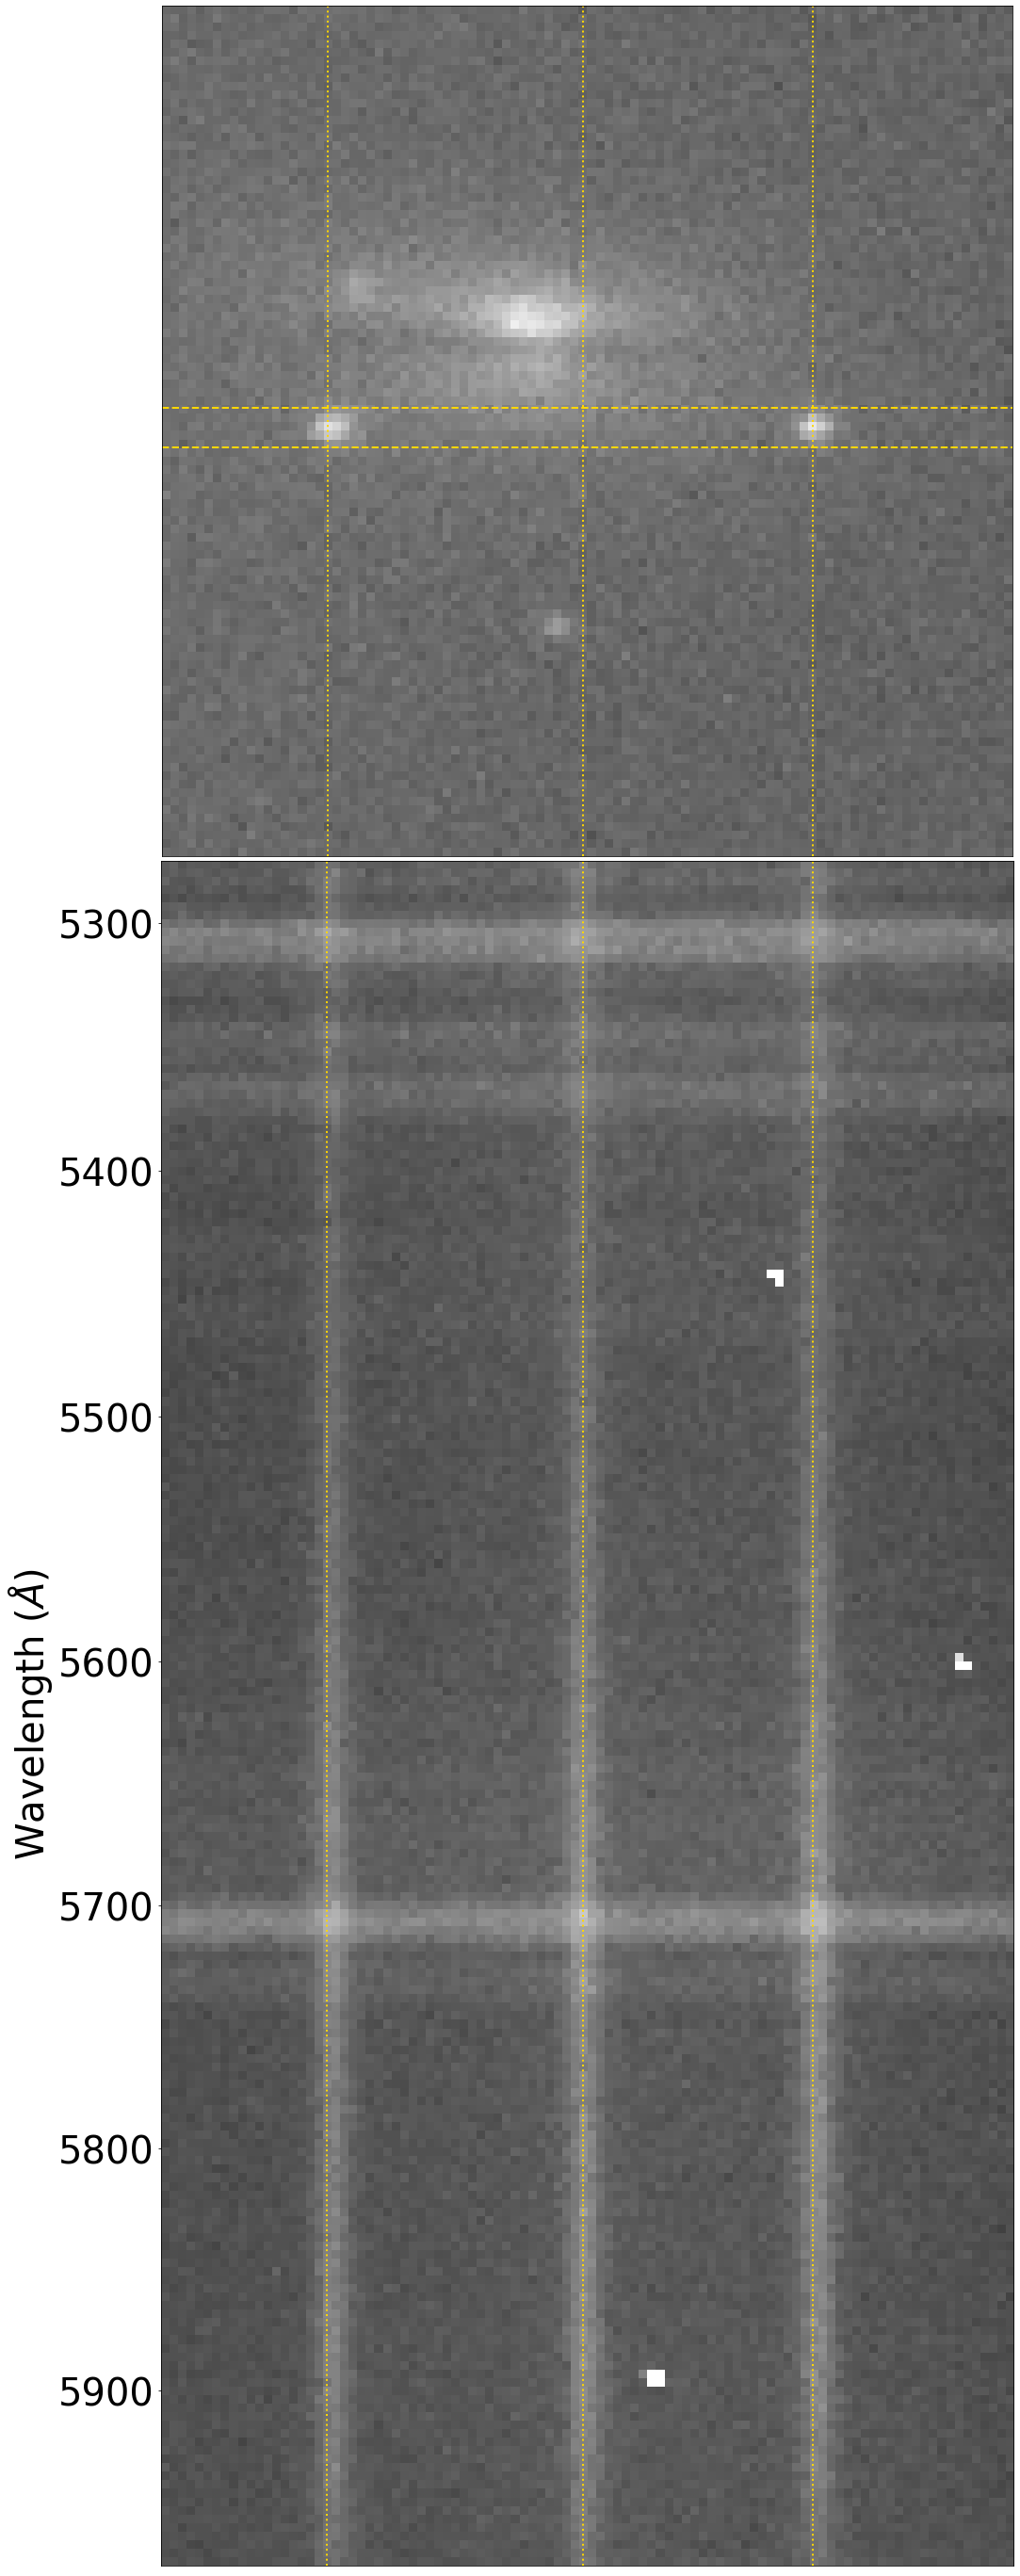
\includegraphics[height=0.8\textheight]{../Images/chapter_2/phot_and_spec_example.png}
    \caption{Image and partial spectrum of SN~2024nqr (left) and SN~2024pgd (right), two SNe Ia active simultaniously in the same galaxy. The image was taken without a filter and used to align the 1.0$\arcsec$ slit (horizontal dashed lines) over both SNe. The resulting spectrum, taken with grism \#4, shows three traces as white vertical stripes. The outer two line up with the two SNe, while the middle trace is from the host galaxy edge in the slit (vertical dotted lines for guidance). The horizontal lines in the spectrum are sky lines coming from atmospheric emission, and the white spots in the spectrum are due to cosmic rays. This data was taken with NOT+ALFOSC on the night of 28 July 2024 while testing an experimental rapid response mode (RRM, credit: Samuel Grund S\o rensen). \color{red}check AT/SN status weirdness \color{black}}
    \label{phot_spec_example}
\end{figure}


Photometry is one of the simplest observing modes as it is just taking a photo of a part of the sky. The top of Fig.~\ref{phot_spec_example} shows a raw photometric image, taken with ALFOSC on the Nordic Optical Telescope (NOT) without the use of a filter. The images are monochromatic, i.e. they only have a value for the intensity. For colourful images multiple observations have to be made using different filters and combined to represent different colours. Faint objects can be observed by increasing the exposure time in a single image, or by stacking multiple images together to increase the effective exposure time. Stacking images can be useful for e.g. reducing cosmic ray interference, avoiding overexposure of a bright source close to a fainter target, or for constructing time series. When stacking images it is common practice to dither the telescope: applying a small offset between exposures to ensure that the target hits a different part of the CCD to avoid issues with bad pixels ruining otherwise good observations. While this decreases the effective size of the fully stacked image, as long as the edges are not needed there is no issue.

\subsection{Spectroscopy}
Spectroscopy goes one step beyond just taking a photo. Assuming that this is slit spectroscopy, instead of a filter to select a wavelength range to observe now a slit restricts the observable region of the sky to a narrow band along one axis of the detector (e.g. horizontal). After the slit the light hits a grating or grism (a grating and prism combined) which diffracts the light based on wavelength across the second axis of the detector (vertical). The rule density on the grating / grism dictates the wavelength spread of the light: the more rules per unit distance, the bigger the diffraction, and the higher the spectral resolution of the resulting image. The tradeoff is that a smaller part of the spectrum can be observed at a time, and there is less light being received per pixel which reduces the SNR unless the exposure time is increased to account for this. Any point-like source that is observed becomes a line in the spectral direction, called a trace. Extended sources create extended traces.

There is some freedom in the orientation of the slit. This is called the position angle of the slit. If there are multiple targets near each other, and they can be in the slit at the same time, the required position angle can be calculated from the two target positions. If there is a single target to be observed the position angle can be anything, but usually the parallactic angle is chosen. In this orientation the slit is perpendicular to the horizon, and prevents losses from differential diffraction (different colours diffracting differently when entering the atmosphere at an angle, \citealt{diff_refrac_atmosphere}). The trace will only be slightly diagonal on the CCD.

The bottom panel of Fig.~\ref{phot_spec_example} shows a section of the spectrum taken of the SNe in the top panel image. The two SNe are drawn out into vertical traces and a third trace belonging to the edge of the host galaxy can be seen in the middle. The horizontal lines are sky emission lines, and while these can technically be used to estimate the conversion from pixel position to wavelength, standardized arc frames will result in a much better wavelength calibration (see section~\ref{reduction}).


\section{Telescopes}
\label{telescopes}
Most of the data used in this thesis comes from the Zwicky Transient Facility (ZTF), and follow-up observations have been made using the Nordic Optical Telescope (NOT), and the Gran Telescopio Canarias (GTC), which will be introduced below. Some additional data comes from other sources, which are listed for completeness. The same filter names (\ztfg\ztfr\ztfi) are used for filters at different telescopes,  which have slight differences. In the rest of this thesis I will use \ztfg\ztfr\ztfi\ to refer to the ZTF filters, unless specified otherwise. \color{red} gotta make sure this is done correctly everywhere \color{black}

\subsection{Zwicky Transient Facility}
\label{ZTF}
The Zwicky Transient Facility (ZTF, \citealt{ZTF_Surveys_Scheduler, ZTF_overview_and_1st_results, ZTF_Science_Objectives, ZTF_Instrumentation, ZTF_Observing_System}) is an optical large-sky survey observing the entire northern night sky above Dec $\approx -30$\degree\ every 2 to 3 nights in three broadband optical filters \ztfg~($\lambda_{eff} = 4746.48$ \AA), \ztfr~($\lambda_{eff} = 6366.38$ \AA), and \ztfi~($\lambda_{eff} = 7829.03$ \AA), which are similar to the well-known SDSS \ztfg\ztfr\ztfi\ filters. The efficiency of these filters is plotted as a function of wavelength in Fig. \ref{Optical_elements_plot}. The survey saw first light in October 2017 and the survey formally began scientific operation in March 2018, and has been running continueously until the time of writing this document.

The observations are made using the $48\arcsec$ aperture Schmidt-type design Samuel Oschin Telescope, which is based at the Palomar Observatory in Southern California. Each exposure is 30 s long, can go a limiting magnitude of $\sim20.5$ mag and covers an area of $\sim47$ deg$^2$ at a resolution of of $1.01\arcsec$ per pixel. The camera is divided in a $4\times4$ grid of CCDs, each of which have 4 readout channels called quadrants. This results in each observation producing 64 separate images, each with their own readout channel identifier (rcid). Similarly, the observed region of the sky is divided into different telescope pointings called fields to ensure that the same region of the sky is observed in the same way each time, aiding with the reduction of the data. This results in each combination of filter, field, and rcid being a set of observations of a particular part of the sky using specific setup.

\begin{figure}
    \centering
    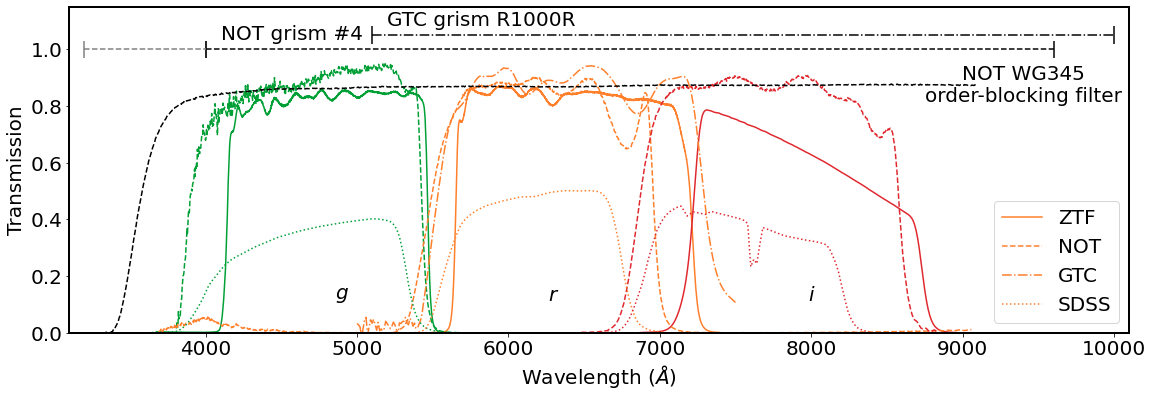
\includegraphics[width=\textwidth]{../Images/chapter_2/transmissions.png}
    \caption{Throughput as a function of wavelength of the different filters used to gather the bulk of the data in this thesis \ztfg\ filters are shown in green, \ztfr\ in orange, \ztfi\ in red, and the different telescopes are shown with different line styles (Continuous for ZTF, dashed for NOT, dot-dashed for GTC). The SDSS filter transmissions (dotted lines) are shown for comparison. For the grisms the wavelength ranges are shown as only, not their efficiency at each wavelength.}
    \label{Optical_elements_plot}
\end{figure}


\subsection{Nordic Optical Telescope}
\label{NOT}
The Nordic Optical Telescope (NOT \footnote{\url{https://not.iac.es}}) is a 2.56 m telescope located at Observatorio Roque de Los Muchacos in La Palma, Spain, at an elevation of 2382 m above sea level. It hosts several instruments for observing in the optical and near infrared, both for imaging and spectroscopy. The \textit{Alhambra Faint Object Spectrograph and Camera} (ALFOSC) was used to obtain the data used in this thesis. I will only discuss the parts relevant to this thesis, further details on this instrument and  details on the other instruments can be found at the NOT website.

ALFOSC is a versatile instrument mounted in cassegrain and can be used for imaging, spectroscopy, and (spectro)polarimtery. As there are several wheels equipped to hold a variety of optical elements, the instrument can switch quickly between different setups between observations. The images can cover up to $6.4\arcmin\times6.4\arcmin$ per exposure at a resolution of $0.2138\arcsec$ per pixel. In this thesis \ztfg~($\lambda_{cen} = 4800$ \AA), \ztfr~($\lambda_{cen} = 6180$ \AA), and \ztfi~($\lambda_{cen} = 7710$ \AA) are used for photometry. For spectroscopy grism \#4 is used to split the light vertically, together with a horizontal $1.0\arcsec$ slit if the seeing was $\leq1.3\arcsec$ or a horizontal $1.3\arcsec$ slit if the seeing was $\geq1.3\arcsec$. Grism \#4 has a resolution of 3.3 \AA\ pixel$^{-1}$ and an wavelength range from 3200 \AA\ to 9600 \AA, but as the response at short wavelengths is poor, the spectra used in this thesis are cut at 4000 \AA. For some spectra an order-blocking filter (WG345) is used as well to avoid second order diffracted blue light to overlap with first order diffracted red light on the detector. The transmission curves of the filters and wavelength range of the grism are shown in Fig.~\ref{Optical_elements_plot}.
%Details on these optical elements are given in Table \ref{NOT_optic_elems}, and they are shown in Fig. \ref{Optical_elements_plot}.

\begin{comment}
\begin{table}
    \centering
    \caption{Optical elements used for observations taken with NOT+ALFOSC and GTC+OSIRIS+. \color{red} Check the $\arcmin$ symbols necessity and make sure to stay consistent \color{black}}
    %\resizebox{\textwidth}{!}{%Scale table to page width
    	\begin{tabular}{ccccc}
    		\hline
    		\hline
    		Filter & $\lambda_\text{center}$ (\AA) & FWHM (\AA) & T$_\text{max}$\\
    		\hline
    		\ztfg$\arcmin$ NOT & 4800 & 1450 & 0.92\\
    		\ztfr$\arcmin$ NOT & 6180 & 1480 & 0.90\\
    		\ztfr$\arcmin$ GTC & 6410 & 1760 & 0.94\\
    		\ztfi$\arcmin$ NOT & 7710 & 1710 & 0.91\\
    		WG345 & 3560 & - & 0.88\\
    		\\
    		\hline
    		\hline
    		Grism & $\lambda$ range (\AA) & resolution (\AA / pixel) & Orientation\\
    		\hline
    		\#4 & 3200$^*$ - 9600 & 3.3 & vertical\\
    		R1000R & 5100 - 10000 & 2.62 & horizontal\\
    		\\
    		\hline
    		\hline
    		slit & Telescope & Orientation\\
    		\hline
    		1.0$\arcsec$ & NOT & horizontal & \\
    		1.0$\arcsec$ & GTC & vertical & \\
    		1.3$\arcsec$ & NOT & horizontal & \\
    		\hline
    	\end{tabular}
    %}
    \begin{flushleft}
    	$^*$ The detector response is limited at low wavelengths, so in practice a lower limit of 4000 \AA\ is used for the spectra in this thesis.
    \end{flushleft}
    \label{NOT_optic_elems}
\end{table}
\end{comment}

\subsection{Gran Telescopio CANARIAS}
\label{GTC}
The Gran Telescopio CANARIAS (GTC \footnote{\url{https://www.gtc.iac.es}}) is a 10.4 m telescope at Observatorio Roque de los Muchachos in La Palma, Spain, and is the largest optical / near infrared telescope on the island. Its primary mirror is made up from 36 hexagonal pieces creating an effective collection area of 73 m$^2$, ideal for observing very faint targets. The GTC can host up to six instruments at a time in various focal positions, allowing for a large variety of observations to be made. One of the most commonly used instruments is OSIRIS+, the upgraded version of OSIRIS: the \textit{Optical System for Imaging and low-Intermediate-Resolution Integrated Spectroscopy}.

OSIRIS+ has an unvignetted field-of-view of $7.8\arcmin\times7.8\arcmin$ at a resolution of $0.254\arcsec$ per pixel. Since the standard readout has $2\times2$ binning, the resolution can be increased to $0.127\arcsec$ per pixel if so desired. Like ALFOSC, this instrument is also built to easily switch between different setups between observations. For photometry the \ztfr~($\lambda_{cen} =6410$ \AA) filter is used in this thesis, and for spectroscopy the R1000R grism with a $1.0\arcsec$ vertical slit is used. R1000R splits the light horizontally over the detector with a range of 5100 \AA\ to 10000 \AA\ with a resolution of 2.62 \AA\ pixel$^{-1}$ These filter transmission curve and grism wavelength range are shown in Fig.~\ref{Optical_elements_plot}.
%Details on the optical elements are given in Table \ref{NOT_optic_elems}, and they are shown in Fig. \ref{Optical_elements_plot}.% ' after the filter?


\subsection{Other observations}
Small amounts of data coming from other telescopes and surveys are presented in this thesis as well. This includes a follow-up observation of SN~2019ldf in Section \ref{sec:late_time_cand} in \ztfg\ and \ztfr\ using the \textit{ESO Faint Object Spectrograph and Camera version 2} (EFOSC2, \citealt{EFOSC2}) imaging spectrograph on the ESO New Technology Telescope (NTT) in La Silla, Chile as part of the extended Public ESO Spectroscopic Survey of Transient Objects+ (EPESSTO+, \citealt{PESSTO}).

To complement ZTF data of several SNe, in chapters \color{red} PUT REFERENCES ONES SECTIONS ARE IN, MIGHT BE DIFFICULT TO DO SECTION SPECIFIC FOR THIS \color{black} optical photometry from the Panoramic Survey Telescope and Rapid Response System (Pan-STARRS, \citealt{Pan-STARRS1}), (intermediate) Palomar Transient Factory (PTF, \citealt{PTF_1, PTF_2}, iPTF, \citealt{iPTF}), All Sky Automated Survey for SuperNovae (ASASSN, \citealt{ASASSN_paper1, ASASSN_catalog}), Asteroid Terrestrial-impact Last Alert System (ATLAS, \citealt{ATLAS}),  and \textit{Global Astrometric Interferometer for Astrophysics} (Gaia, \citealt{Gaia}) are used, as well as near-infrared photometry from the \textit{Wide-Field Infrared Survey Explorer} (WISE, \citealt{WISE}).


\section{Calibration images}
\label{calibration}
Before the observations can be used for science, the images need to be calibrated. This is done using different types of calibration images, each of which measure and correct for different effects of the telescope and detector. Usually these are taken during the day or twilight so no valuable observing time is lost. It is standard practice to take multiple calibration images and use an odd number in the reduction to find median values and remove interference from e.g. cosmic rays, this is called a master image.


\subsection{Bias}
The first type of calibration image is the bias, which is made by reading out the CCD without exposing. The resulting image contains the amount of counts that will be in every exposure regardless of what has been observed or with what exposure time. In other words, measuring the bias can be tought of as measuring the offset to correct for in every other image.

%$B_{ij}$ is the so-called bias, the measured pixel response that is in every observation regardless of the exposure time and amount of light hitting the pixel. The easiest way to measure this value is to take bias frames: observe with an exposure time of 0 with no light hitting the CCD. $F$ and $t$ are 0 which reduces Eq.~\ref{CCD_response} to $R_{ij}(0, 0) = B_{ij}$

\subsection{Dark}
Any detector that is not at a temperature of 0 K will have some amount of noise due to thermal effects. This can free electrons in pixels over time, creating a dark current and increasing the noise over time. The effect can be measured by exposing for the same amount of time as the science images taken, but without letting any light hit the CCD. This is called a dark frame.

As this is a thermal effect, it can be reduced to negligible amounts by cooling the instrument. This saves precious observing time, as otherwise dark frames would ideally have to be taken at the same temperature as the target was observed, which is easiest to do directly after the science exposure. By cooling the detector with e.g. liquid nitrogen this noise source can be avoided instead of having to correct for, saving time and the amount of images that need to be taken in the process.

%Next is $D_{ij}$, the noise that increases with longer exposure times. This is thermal noise, and as its name suggests it is more impactful the higher the temperature $T$ is in the CCD: $D_{ij} = D_{ij}(T)$. Due to this there are actually two ways to remove this source of noise. One can take Dark frames by exposing for some amount of time but making sure no light hits the detector, $R_{ij}(0, t) = B_{ij} + D_{ij} \times t$, and extract $D_{ij}$. This takes however a lot of time, and it is often more efficient to cool the CCD down to very low temperatures (e.g. with liquid nitrogen) to ensure $D_{ij}$ can be neglected.

\subsection{Flatfield}
The amount of light that the telescope receives is converted into a digital number, but there is no guarantee that this conversion rate is the same for each pixel. This can be due to intrinsic differences between the pixels, or outside effects such as dust reducing the amount of light recieved on a part of the detector. To correct for this an evenly illuminated field has to be observed, resulting in an image called a flat or flatfield. By ensuring that each pixel receives the same amount of light, the different counts will reflect the varying responses per pixel.

Any evenly illuminated object can be used for this, such as the the inside of the telescope dome to create dome flats. A more perfect evenly lit source however is the sky, and using this sky flats can be taken. While it is usually too bright during the day and the CCD will saturate even with the narrowest filter and shortest exposure time, there is a window during twilight where the sky is darker but not dark enough to observe stars yet, perfect for taking flats. As a general rule, narrowband filters need a brighter sky and in the evening these need to be done before the broadband filters. After that, assuming similar efficiencies between filters, blue filters need brighter skies than red filters, forcing a specific order in which the sky flats need to be taken during the short window where this is possible. Of course if flats are taken in the morning the order has to be reversed.

%Lastly, to measure $A_{ij}$ flatfield images are needed. During a science exposure the amount of light hitting a pixel is dependent of the brightness of the source at that location, $F = F_{ij}$. But as not every pixel may have the same response the measured values need to be normalized before different pixels can be compared. This is done by observing an evenly lit background where $F_{ij}$ is the same for every pixel. This can be done by observing the inside of the dome (dome flats), although the twilight sky (sky flats) are usually preferred as they are more evenly lit across the CCD.

\subsection{Arc}
In spectroscopy one of the axes has low wavelength at one end and high wavelength at the other end of the image. To know where each wavelength falls on the detector, arc frames are needed. These are taken by observing a lamp filled with a known set of elements (e.g. He, Ne, or TH and Ar). The wavelengths of the emission lines are known very precisely, and by matching these with the observed lines in the arc image a pixel-to-wavelength conversion can be found, called the wavelength solution.

Usually arcs can be taken during the day, when the telescope is idle. However in some cases the mechanical flexure of the telescope, caused by being in a different position during observing, can introduce an uncertainty in the wavelength calibration unless an arc is taken with the telescope in the same position as for the target. In these cases an arc is usually taken directly before or after the target is observed, or between exposures of the target.

%For spectroscopy another type of calibration is needed: Wavelength calibration. This is done with arc frames: observing the known emission lines of several elements using lamps in the instrument (e.g. He, Ne, ThAr lamps) using the same setup as the science observation. The resulting pattern of emission lines is known and can be used to map the pixel position in the spectral direction to a wavelength, called the wavelength solution.

\section{Reduction}
\label{reduction}
After all observations have been taken it is time to analyze them. The first step is to reduce the raw data into the required format to work with. After that, additional analysis technique can manipulate the reduced images directly or the data that has been extracted from them. The response function of a detector can be written as

\begin{equation}
	R_{ij}(f, t, \lambda) = B_{ij} + D_{ij}(t) + F_{ij}(\lambda) \times f \times t,
	\label{CCD_response}
\end{equation}

where $R_{ij}$ is the CCD response of pixel $i,j$ as a function of the integrated flux of the target $f \times t$ during the exposure which lasted a time $t$. The goal is to measure the flux $f$, which requires knowing and correcting for the bias level $B_{ij}$, dark current $D_{ij}$, and pixel response $F_{ij}$. Each type of calibration image is used to measure one of these values. Note that it is assumed that there are no cross or higher order terms in Eq.~\ref{CCD_response}, in other words, the CCD is in its linear regime. When a pixel receives too much light and gets close to saturation it is no longer in its linear regime, and more terms appear in Eq.~\ref{CCD_response} making it much more difficult or even impossible to measure the observed flux.


\subsection{Bias, dark, and flat corrections}
Using the calibration images from section~\ref{calibration}, the raw science images can be reduced to something a flux level can be measured from. 

First the master-bias is created and subtracted from every other image. As both $F$ and $t$ are 0, the bias measures $B_{ij}$ directly and can then immediately be removed.

With the bias gone, the dark frames measure $D_{ij}$ for a specific $t$, but the master-dark can only be used on sciene observations with the same exposure time. Alternatively it is possible to subtract $B_{ij} + D_{ij}(t)$ in a single step by not separating out the bias term using bias images first.

Finally every science image is divided through the normalized master-flat to equalize the pixel responses. There is still a factor $F(\lambda)$ present as the detector efficiency is wavelength dependent, but the value is now indepentent of the pixel position, allowing values from across the CCD to be compared.

\subsection{Cosmic-ray removal and image stacking}
At this point it is often good practice to run a cosmic-ray removal algorith to remove this source of noise as much as possible. This can be done using e.g. L.A.Cosmic \citep{lacosmic}, which I used through Astro-SCRAPPY \citep{astroSCRAPPY} when reducing follow-up photometry of several objects in this thesis.

If multiple images are taken of the same field or object they can be stacked to reduce background noise and increase the SNR of the observed objects. Sometimes the observations have been taken with dithering to avoid the same objects being on the same pixels in every exposure, which has to be taken care of to make sure that the images are stacked correctly.

\subsection{Standard star calibration}
Filters are never 100\% transparent at any wavelength, and the CCD responds differently to different wavelengths as well. To correct for this, one last type of calibration image is used: the standard star. This was not mentioned in section~\ref{observation_types} as observing a standard star is exactly the same as observing the actual science target. The only difference is that the expected result of the observation is known and can be used to correct for the wavelength depent efficiency of the instrument.

With photometry the observed brightness can be measured for each star in the image to get a list of instrument magnitudes. The relative differences between the magnitudes of objects are correct, but there is still an absolute offset across all objects. This is corrected by finding the offset using the standard star. If the filter is commonly used, there is a good chance many stars in the field have known magnitudes in that filter, which can be used for calibration instead of a dedicated standard star.

In spectroscopy the arcs are used to find the wavelength solution for the spectra, after which the trace from the standard star can be extracted and divided by the known spectrum of the star to obtain the sensitivity function of the detector $F(\lambda)$. The trace of the target can be extracted as well to get its spectrum, which can then be flux-calibrated using the sensitivity function. In some cases only a relative sensitivity function is known, resulting in a calibrated spectrum in an unknown flux unit. In these cases proper calibrated photometry of the obect can be used to flux-calibrate the spectrum by integrating the spectrum over the filter transmission curve.


\begin{comment} %USE IMAGE ELSEWHERE?
\subsection{Difference imaging}
Transients are, by definition, objects that appear on the sky for a limited amount of time. A popular and effective way to search for new objects is difference imaging. If there is a map or image of how a part of the sky looked some time ago, it can be used as a reference and subtracted from an image of the current sky. Constant sources such as most stars and galaxies (except variable ones) can be removed. To computers images are nothing more than big matrices. This means that, if properly aligned, subtracting the reference from the science images is an easy operation that leaves only those sources whose brightness has changed between the two observations in the so-called difference image. This also ensures that only the transient light is measured in cases where different sources are superimposed, such as a SN superimposed on top of its host galaxy. Figure~\ref{diff_im_example} shows an example of the resulting difference image after subtracting the reference image from the science image.

\begin{figure}
    \centering
    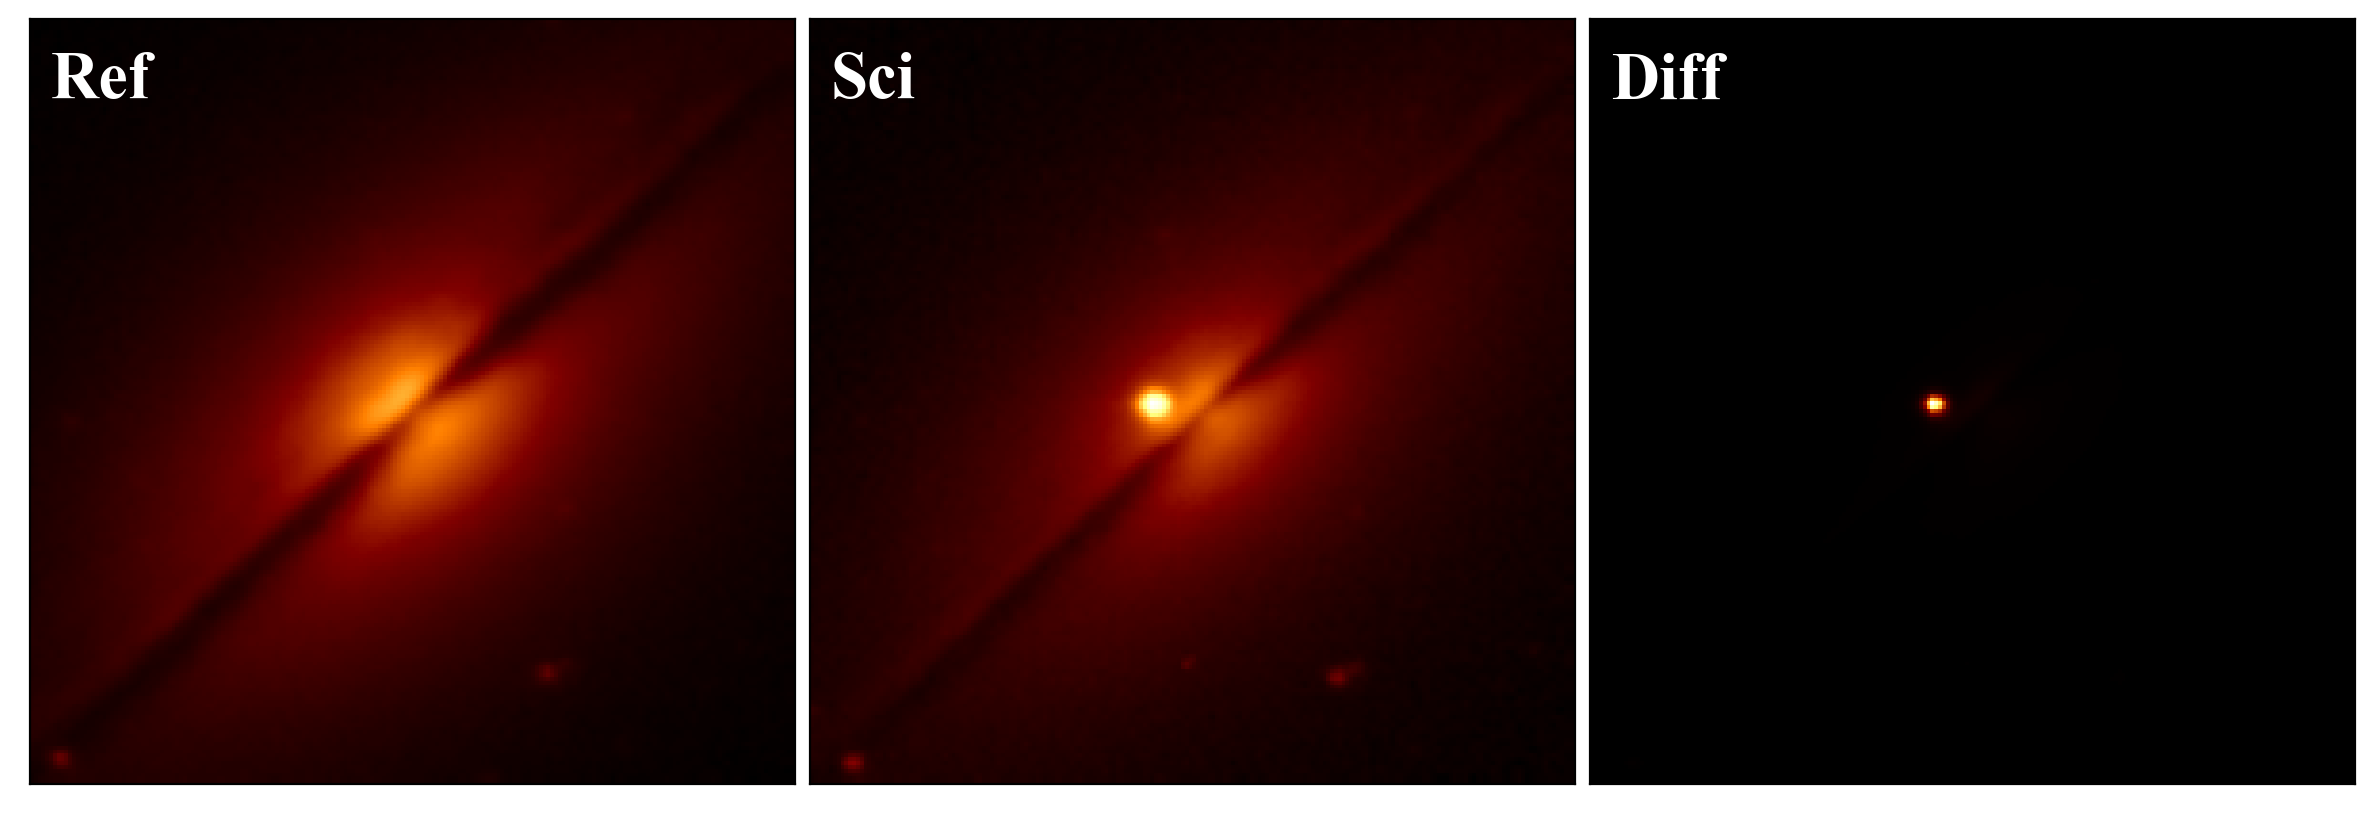
\includegraphics[width=\textwidth]{../Images/chapter_2/diff_im_SN2021rhu.png}
    \caption{Example of a \ztfr-band reference image of NGC 7814, the science image of the same region, and the resulting difference image with the host galaxy removed and only the transient (SN~2021rhu, SN Ia 86G-like) remaining. Credit: Luke Harvey}
    \label{diff_im_example}
\end{figure}
\end{comment}

\subsection{Forced photometry}
The two most common methods to measure flux from as source in an photometric image are PSF photometry and aperture photometry. A good explanation of these can be found in \citet{Photometry_techniques}. PSF stands for point spread function, and with this method a function is fitted to model the source. This function describes how an infinitely small point of light is spread over the detector, and through its spatial size and peak value the flux of the light source can be measured. Aperture photometry sums up the signal in a given radius around the source center and subtracts the contribution from the background in the same region.

%\color{red} See \url{https://coolwiki.ipac.caltech.edu/index.php/Aperture_Photometry_Overview} for references \color{black}

Large surveys such as ZTF observe the night sky to find new transients and monitor known ones. Difference imaging is used to subtract constant sources and reveal active transients, as these are the main sources that should be left in the difference image along with solar system objects that move across the sky. A historically popular algorithm for difference imaging is High Order Transform of PSF ANd Template Subtraction (\textsc{hotpants}, \citealt{HOTPANTS})\footnote{\url{https://github.com/acbecker/hotpants}}, which is used for image subtraction in Sect.~\ref{sec:late_time_cand}. There are other algorithms as well. For instance, ZTF uses \textsc{zogy} \citep{ZOGY}\footnote{\url{https://github.com/cenko/ZOGY}}, and in \color{red}Sect. \color{black} \textsc{autophot} \citep{Autophot}\footnote{\url{https://github.com/Astro-Sean/autophot}} is used to subtract reference images from follow-up observations obtainted with the NOT and GTC.

Through PSF photometry the location and strength of each source in the image is determined, which are then compared to the locations of known sources to separate new from known ones. Each location has however been observed for the entire duration of the survey, which means that it is also possible to measure the flux of a known transient before and after it was visible in the images, creating a light curve for the full duration of the survey.

This is called forced photometry, because the PSF function is forced to center on a specific location instead of finding the best-fitting position for the centroid. All ZTF light curves that are used in this thesis have been obtained through \textsc{fpbot} \citep{fpbot}\footnote{\url{https://github.com/simeonreusch/fpbot}}. When there is nothing but noise at that location the measured flux will be 0 within the error. When there is a source at the target location it will be measured, but if the source is not at the center of the PSF the fit will have trouble converging, resulting in a large uncertainty. Artefacts such as cosmic rays, imperfectly subtracted difference images, or light bleeding effects from saturated bright nearby stars can also affect the accuracy of the photometry measurement.

%\section{The SuperNova Animation Program}
%The light curve that is the result of applying forced photometry at a specific location for the entire run of a survey can contain bad data points. Many of these will be flagged for having a bad PSF fit, bad weather conditions, etc. But even after filtering these out it can be helpful to check the difference images themselves for unexpected behavouir that might be captured in the light curve. For this I created the SuperNova Animation Program (\textsc{snap} \footnote{\url{https://github.com/JTerwel/SuperNova_Animation_Program}})

%\textsc{snap} collects image cutouts of the specified location during the  specified time period(s) and in the specified filter(s). It then matches these with the individual data points in the light curve and puts the images in an animation in chronological order with the reference images at the start. This enables easy identification of bad points due to image defects, off-center sources, residual from imperfectly subtracted sources, cosmic rays etc.

%\section{Simulations}
%Some experiments are difficult or even impossible to do multiple times, one cannot rerun a survey to observe the same transient events. So to understand the biases in the data as well as the effective size of the survey, it needs to be simulated. I used \textsc{simsurvey} \citep{simsurvey,simsurvey_main} \footnote{\url{https://github.com/ZwickyTransientFacility/simsurvey/tree/master}} to simulate an observing campaign like ZTF detecting a specific event under different circumstances. For \textsc{simsurvey} to work both the observer and observed have to be specified, i.e. a model of the telescope, observatory, and survey is required, as well as a model of the transient and where to place it. More details on how the simulation is run are given in section \color{red}ref to paper 1 sim section \color{black}


\section{General considerations for observing}
\label{considerations}
During my PhD I have spent two years doing studentships with the Isaac Newton Group of Telescopes (ING) and Nordic Optical Telescope (NOT) on La Palma, gaining first-hand experience with the specifics of observing in the optical regime and the considerations that come with it. I will briefly go over these in this section. These studentships also gave me the unique opportunity to very quickly follow up on interesting transients, which was very valuable for the objects that will be discussed in \color{red}chapter\color{black}.

%To observe astronomical objects one has to consider several things. Assuming that the location or region on the sky to target is already known, as well as what type of data to collect, an observing plan can be made. A well constructed observing plan should allow to obtain the best quality data possible while making efficient use of the resources available.


\subsection{Location}
Although this is normally already done before constructing a telescope, the first thing to consider is the observing location. When purely aiming for the best observations possible, there are three main things to consider when choosing where to observe from:
\begin{itemize}
    \item {Weather: Clear, stable sky conditions for most nights of the year, and low atmospheric distortion (e.g. seeing) are vital to ensure good quality data on a regular basis. Low hanging clouds can be avoided by being high above sea level, while simultaneously decreasing the amount of air light has to travel through to reach the detector, decreasing atmospheric influence.}
    \item {Light pollution: Darker skies allow observations of fainter objects. Even the the presence of a (partially) illuminated moon significantly changes the depth that can be reached with the same exposure time. Many observatories have (inter)national laws to control the ligth pollution and ensure good quality data can be obtained.}
    \item {Target observability: The target location needs to be reachable by the telescope to be observable. The closer to zenith an observation is made, the less atmosphere between the target and telescope. The atmosphere reduces the data quality through turbulence (seeing), broadband absorbtion (clouds, dust), narrowband interference (tellurics, skylines), and differential diffraction, among others.}
\end{itemize}

Observatories should be located on top of high mountains in areas with stable and clear weather, with as small a nearby population as possible while still being accessible enough for transporting materials and observing staff. One of the best locations in the world that meets these requirements is Roque de los Muchachos on La Palma, a small Spanish island in the Atlantic ocean off the coast of Morocco. At around 2300 m above sea level, the telescopes are built on the highest peak of the mountain far from most communities on the island which are much closer to sea level, and the temperate climate ensures good sky conditions for most nights around the year. Additionally, the government has put laws in place to minimize light pollution, e.g. by limiting the use of street lights and restricting flight paths over the island. \color{red} I remember a plaque at the roque mentioning this, maybe it has a good ref? \color{black}


\subsection{Telescope, instrument, observation type, and setup}
Depending on the type of observations and the brightness of the target there is a choice of hardware to be used. Telescope, intsrument, observation type, and desired setup(s) have to be considered together, as some choices will affect other ones.

Bigger telescopes can observe fainter targets, but it is also more difficult to obtain observing time. On the other hand, smaller telescopes are less oversubscribed (a measure of requested versus available observing time), but are more limited in observation depth even with long exposure times. %Small telescopes are however ideal for bright targets that would instantly saturate the detector of a larger telescope if no filter was used.

Secondly, different instruments, which are often telescope specific, have different observing capabilities. Photometry and spectroscopy are very standard observing modes, and most telescopes have at least one instrument can offer this. Even though ALFOSC and OSIRIS+ can both of these modes, there are still differences in data quality and resolution even if the same object is observed at the same time. However for polarimetric observations for instance, OSIRIS+ cannot be used while ALFOSC can, limiting the options for this observation mode.

Lastly, the specific setup has to be considered as well. For photometry, which filters are desired? If a very specific or rare filter is needed this may limit the options of telescopes and instruments. For spectrocopy there are other choices, such as fiber or slit spectroscopy, different gratings or grisms depending on the desired resolution and wavelength range, neutral density filters to observe targets that are otherwise too bright for the instrument, and order-blocking filters to remove second order blue light from red parts of the spectrum.


\subsection{Night plan}
Lastly, it is good to have a plan of what to observe at each point during the night in order to avoid losing observing time during the night. Most proposals already have a list of targets and standard stars to observe and exposure times when they are submitted to request observation time, but the detailed plan is usually made mere hours before the night starts as it depends on e.g. the current weather, target priority, and specific time constraints (e.g. for transits). Calibration images might need to be taken during the night as well. All of these things need to be concidered when trying to maximize the time used to expose and observe targets, and minimize the overheads from e.g. positioning, target acquisition, and readout.

Time spent repositioning the telescope can be reduced by finding the path between targets that minimizes telescope and dome movement throughout the night. The target acquisition time depends on the type of observation, but also on the experience and tiredness of the observer. With photometry a field is observed, so usually a small offset is not disastrous for the science. With spectroscopy the target needs to be identified and placed in the slit or fiber before the exposure can start, costing extra time. Readout times are detector specific, but can be sped up by windowing and binning if only a part of the CCD is needed, and a worse resolution is acceptable. Considering readout times can be especially important when multiple shorter exposures are taken instead of a single long one.

Nothing is certain during the night. Weather conditions can change suddenly, technical problems can occur, a high priority target can be discovered during the night, or observations might go so smoothly that they are completed faster than expected. A flexible schedule with a priority list and backup targets helps adapting to these situations quickly. After all, an idling telescope in (half-)decent observing conditions is a waste of resources. Fig.~\ref{visplot} shows an example night plan for the NOT with some space for adaptibility built in.

\begin{figure}
    \centering
    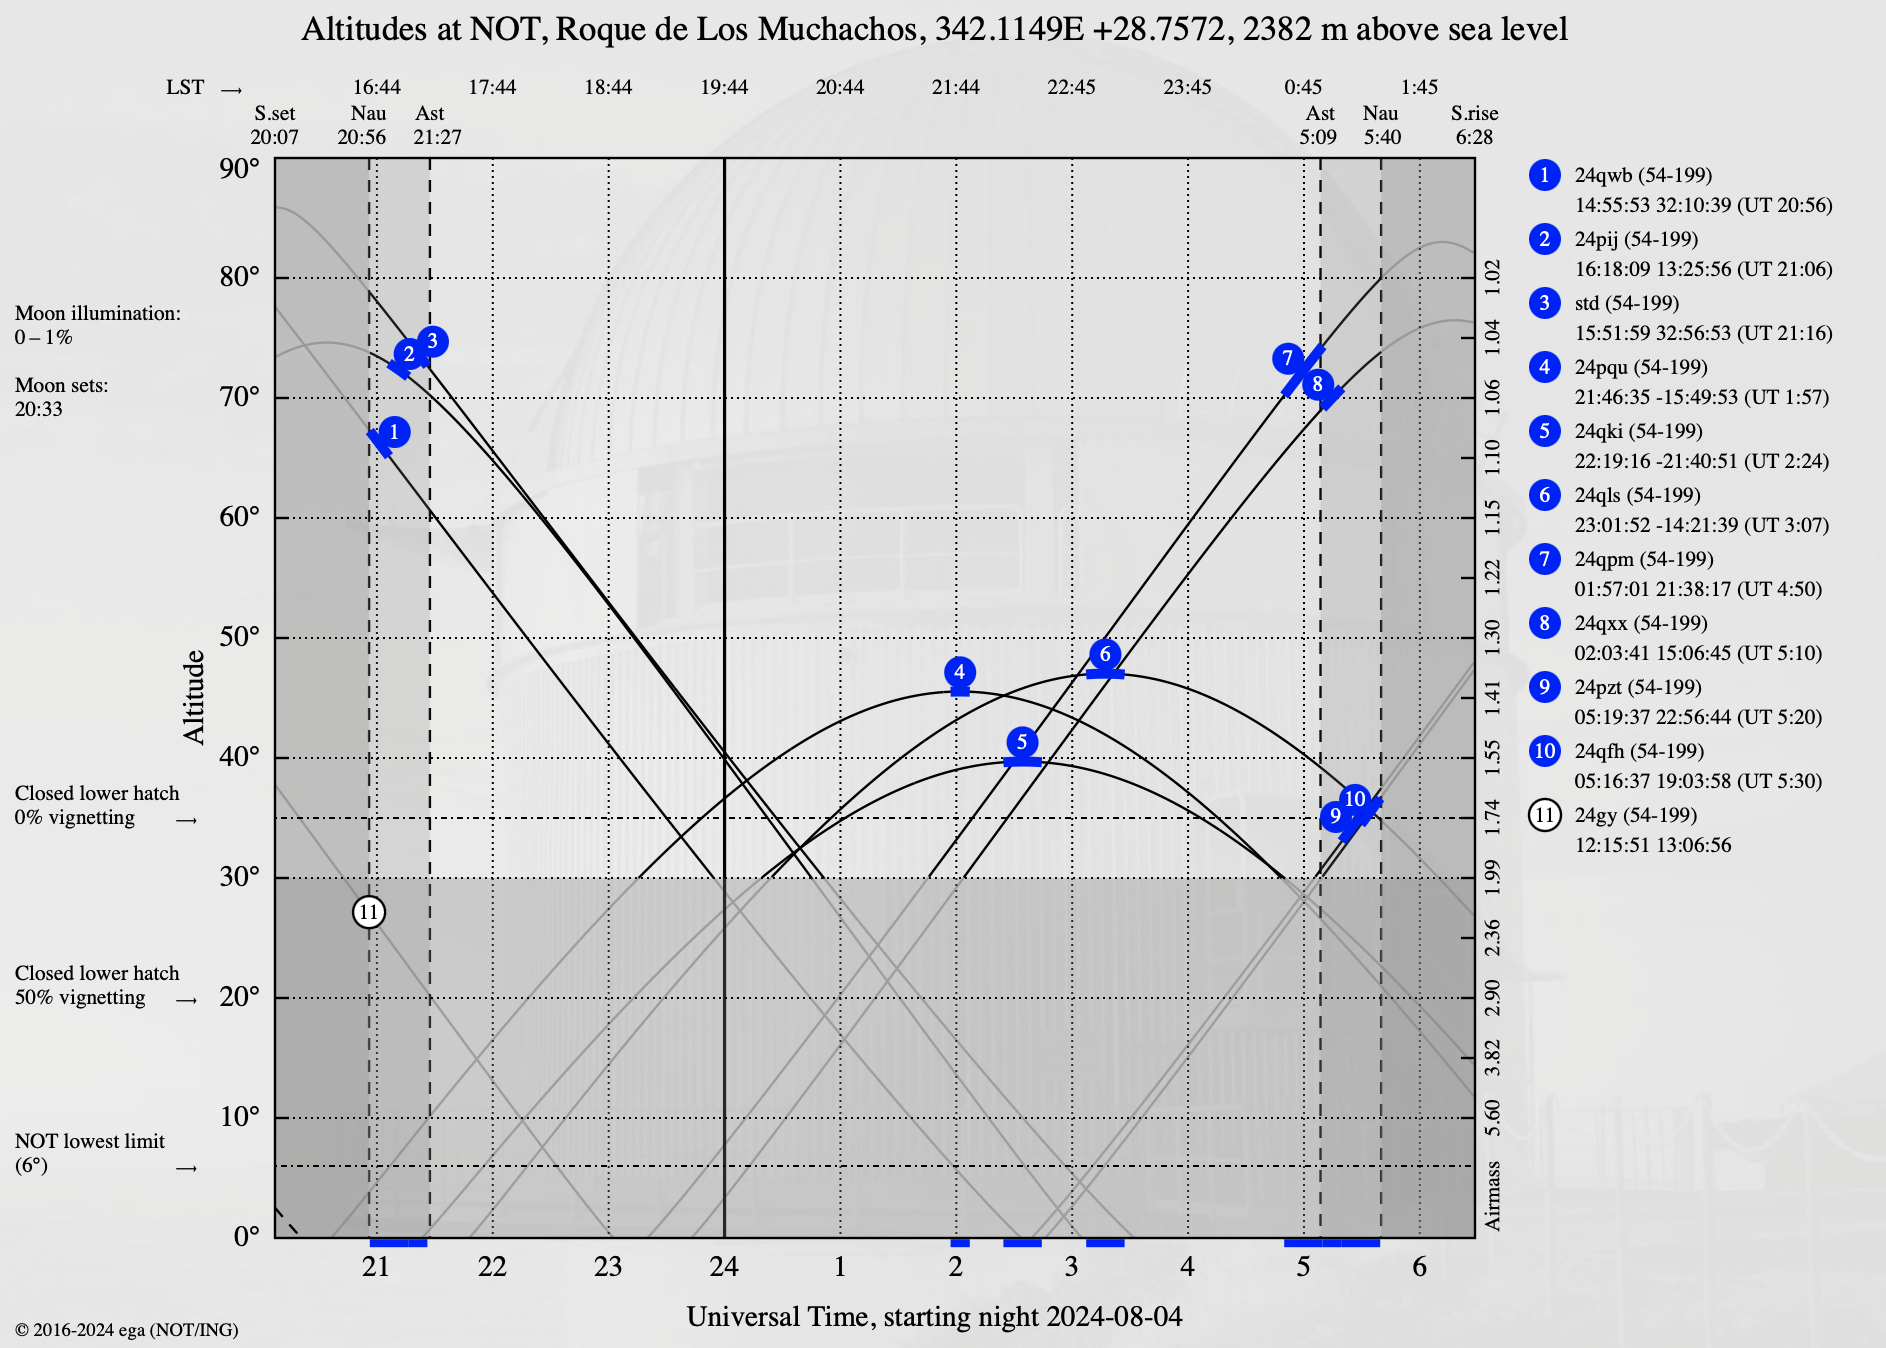
\includegraphics[width=0.95\textwidth]{../Images/chapter_2/visplot.png}
    \caption{Night plan for the NOT on the night of 10 August 2024. Targets are plotted with their altidute as a function of universal standard time. Local stellar time is shown on top. The target priority has been colour coded, with the coloured bars showing the amount of time each observation is expected to take. Green targets have already been completed, and the red vertical line shows the current time. Several unscheduled backup targets are shown in case the plan has to be updated during the night.}
    \label{visplot}
\end{figure}



\end{document}
%!TEX root = ../main.tex
\documentclass[a4paper,oneside,12pt, class=Latex/Classes/PhDthesisPSnPDF, crop=false]{standalone}
\usepackage{setspace}
\begin{document}
\doublespacing
\chapter{Analysis techniques}
\label{chap:analysis}


\color{red} This chapter has been absorbed into the observing chapter \color{black}

\end{document}
% --------------------------------------------------------------
%:                  BACK MATTER: appendices, refs,..
% --------------------------------------------------------------

%: ----------------------- bibliography ------------------------

\newgeometry{left=1.6cm, right=1.6cm, top=1.0cm, bottom=1.0cm, footskip=0cm}
\singlespacing
%\begin{footnotesize} 
\bibliographystyle{aa}%{plainnat}
\renewcommand{\bibname}{References} 
%\begin{multicols}{2}

\bibliography{thesis_references}

%\end{multicols}

\singlespacing
%\end{footnotesize}
\restoregeometry

\appendix
%\include{appendix/app}


\end{document}